% Default font is 11pt, which is pretty big, especially for internal
% talks Default aspect ratio is 4:3. "32", i.e. 3:2, is a compromise
% between 4:3 and 16:9
%
% Compromising on 3:2 is reasonable when you're going to show the talk
% on a projector and you don't know what kind of projector or screen it
% will be.
%
% 16:9 is best if others will be viewing it on their own devices,
% fullscreen.
%
% 4:3 is best if others will be viewing it on their own devices in a
% meeting where they want to also see the participants list/participant
% video/chat window.
%
% 3:2 is a good compromise when people will be viewing it on their own
% devices, but you don't know if they'll want to use part of the screen
% for something else or not.
%
% So 3:2 is the best default overall as of 2021. This may well change in
% the future.
%
\documentclass[aspectratio=32,10pt]{beamer}

% These together produce the same font as usual, but with copyable underscores
\usepackage[T1]{fontenc}

\usepackage{xspace}
\usepackage[absolute, overlay]{textpos}
\usepackage{verbatim}
\usepackage{graphicx}
\usepackage{array}

% Sets default width for includegraphics images
\setkeys{Gin}{width=\columnwidth}

\frenchspacing

\hypersetup{colorlinks}

\newcommand{\ul}{\begin{itemize}}
\newcommand{\lu}{\end{itemize}}
\newcommand{\ol}{\begin{enumerate}}
\newcommand{\lo}{\end{enumerate}}

\newcommand{\cols}{\begin{columns}}
\newcommand{\sloc}{\end{column}\end{columns}}

\newcommand{\col}{\begin{column}{0.5\textwidth}}
\newcommand{\colw}[1]{\begin{column}{#1\textwidth}}

\newcommand{\colbr}{\end{column}\begin{column}{0.5\textwidth}}
\newcommand{\colbrw}[1]{\end{column}\begin{column}{#1\textwidth}}

\newcommand{\hl}{$t_{1/2}$\xspace}

\newcommand{\is}[2]{\texorpdfstring{${}^{#1}$#2}{#2-#1}}

\newcommand{\meas}[4]{$(#1#2\mathrm{(stat)}#3\mathrm{(syst)})#4$}

\newcommand{\cn}{$^{\mathrm{[citation~needed]}}$\xspace}

\newcommand{\dedx}{$\mathrm{d}E/\mathrm{d}x$\xspace}
\newcommand{\piz}{$\pi^0$\xspace}
\newcommand{\pip}{$\pi^+$\xspace}
\newcommand{\pim}{$\pi^-$\xspace}
\newcommand{\mup}{$\mu^+$\xspace}
\newcommand{\mum}{\texorpdfstring{$\mu^-$\xspace}{mu\xspace}}

% "bold all" -- make both normal and math mode bold
\newcommand{\ba}[1]{{\boldmath \bf #1}}


\setbeamertemplate{navigation symbols}{} 
\mode<presentation>

% With minimal space usage for sections:
% default
% Boadilla
% Madrid
% Pittsburgh
% Rochester
%
% With space used at top for sections:
% AnnArbor
% Antibes
% Berlin
% CambridgeUS
% Copenhagen
% Darmstadt
% Dresden
% Frankfurt
% Ilmenau
% JuanLesPins
% Luebeck
% Montpellier
% Singapore
% Szeged
% Warsaw
%
% With space used on right or left for sections:
% Berkeley
% Goettingen
% Hannover
% Malmoe
% Marburg
% PaloAlto
%
% With space used on left for ... something:
% Bergen
\usetheme{PaloAlto}
% default
% albatross
% beaver
% beetle
% crane
% dolphin
% dove
% fly
% lily
% orchid
% rose
% seagull
% seahorse
% whale
% wolverine
\usecolortheme{default}

\setbeamersize{text margin left=2mm,text margin right=2mm} 

\author{Matthew Strait}
\institute{University of Minnesota}

%%%%%%%%%%
% Tricks %
%%%%%%%%%%

\newcommand{\beginbackup}{
   \newcounter{framenumbervorappendix}
   \setcounter{framenumbervorappendix}{\value{framenumber}}
}
\newcommand{\backupend}{
   \addtocounter{framenumbervorappendix}{-\value{framenumber}}
   \addtocounter{framenumber}{\value{framenumbervorappendix}} 
}

\newcommand{\topbit}[3]{
  \title[#3]{#1}
  \pdfinfo{
     /Author (Matthew Strait)
     /Title  (#1)
  }
  \date{#2}

  \begin{document}

  \frame{
   \maketitle
  }

}

\usepackage{tikz}

\newcommand{\hcancel}[1]{%
    \tikz[baseline=(tocancel.base)]{
        \node[inner sep=0pt,outer sep=0pt] (tocancel) {#1};
        \draw[black] (tocancel.west) -- (tocancel.east);
    }%
}%

\setbeamertemplate{footline}[frame number]


\topbit{LIGO/Virgo follow-up progress}{23 Feb 2018}
       {GW, LIGO}

\section{Intro}

\frame{\frametitle{Introduction}

\ul

\item LIGO/Virgo (LVC) has reported 7 gravitational wave events

\item 6 black hole mergers (starting to be routine!)

\item 1 neutron star merger

\item One of each with Virgo online: good pointing

\item Other possible signals: supernovae, exotics

\item We should report on whether we saw anything coincident
with any of these

\lu

}


\frame{\frametitle{Black hole/black hole mergers}

\begin{center}
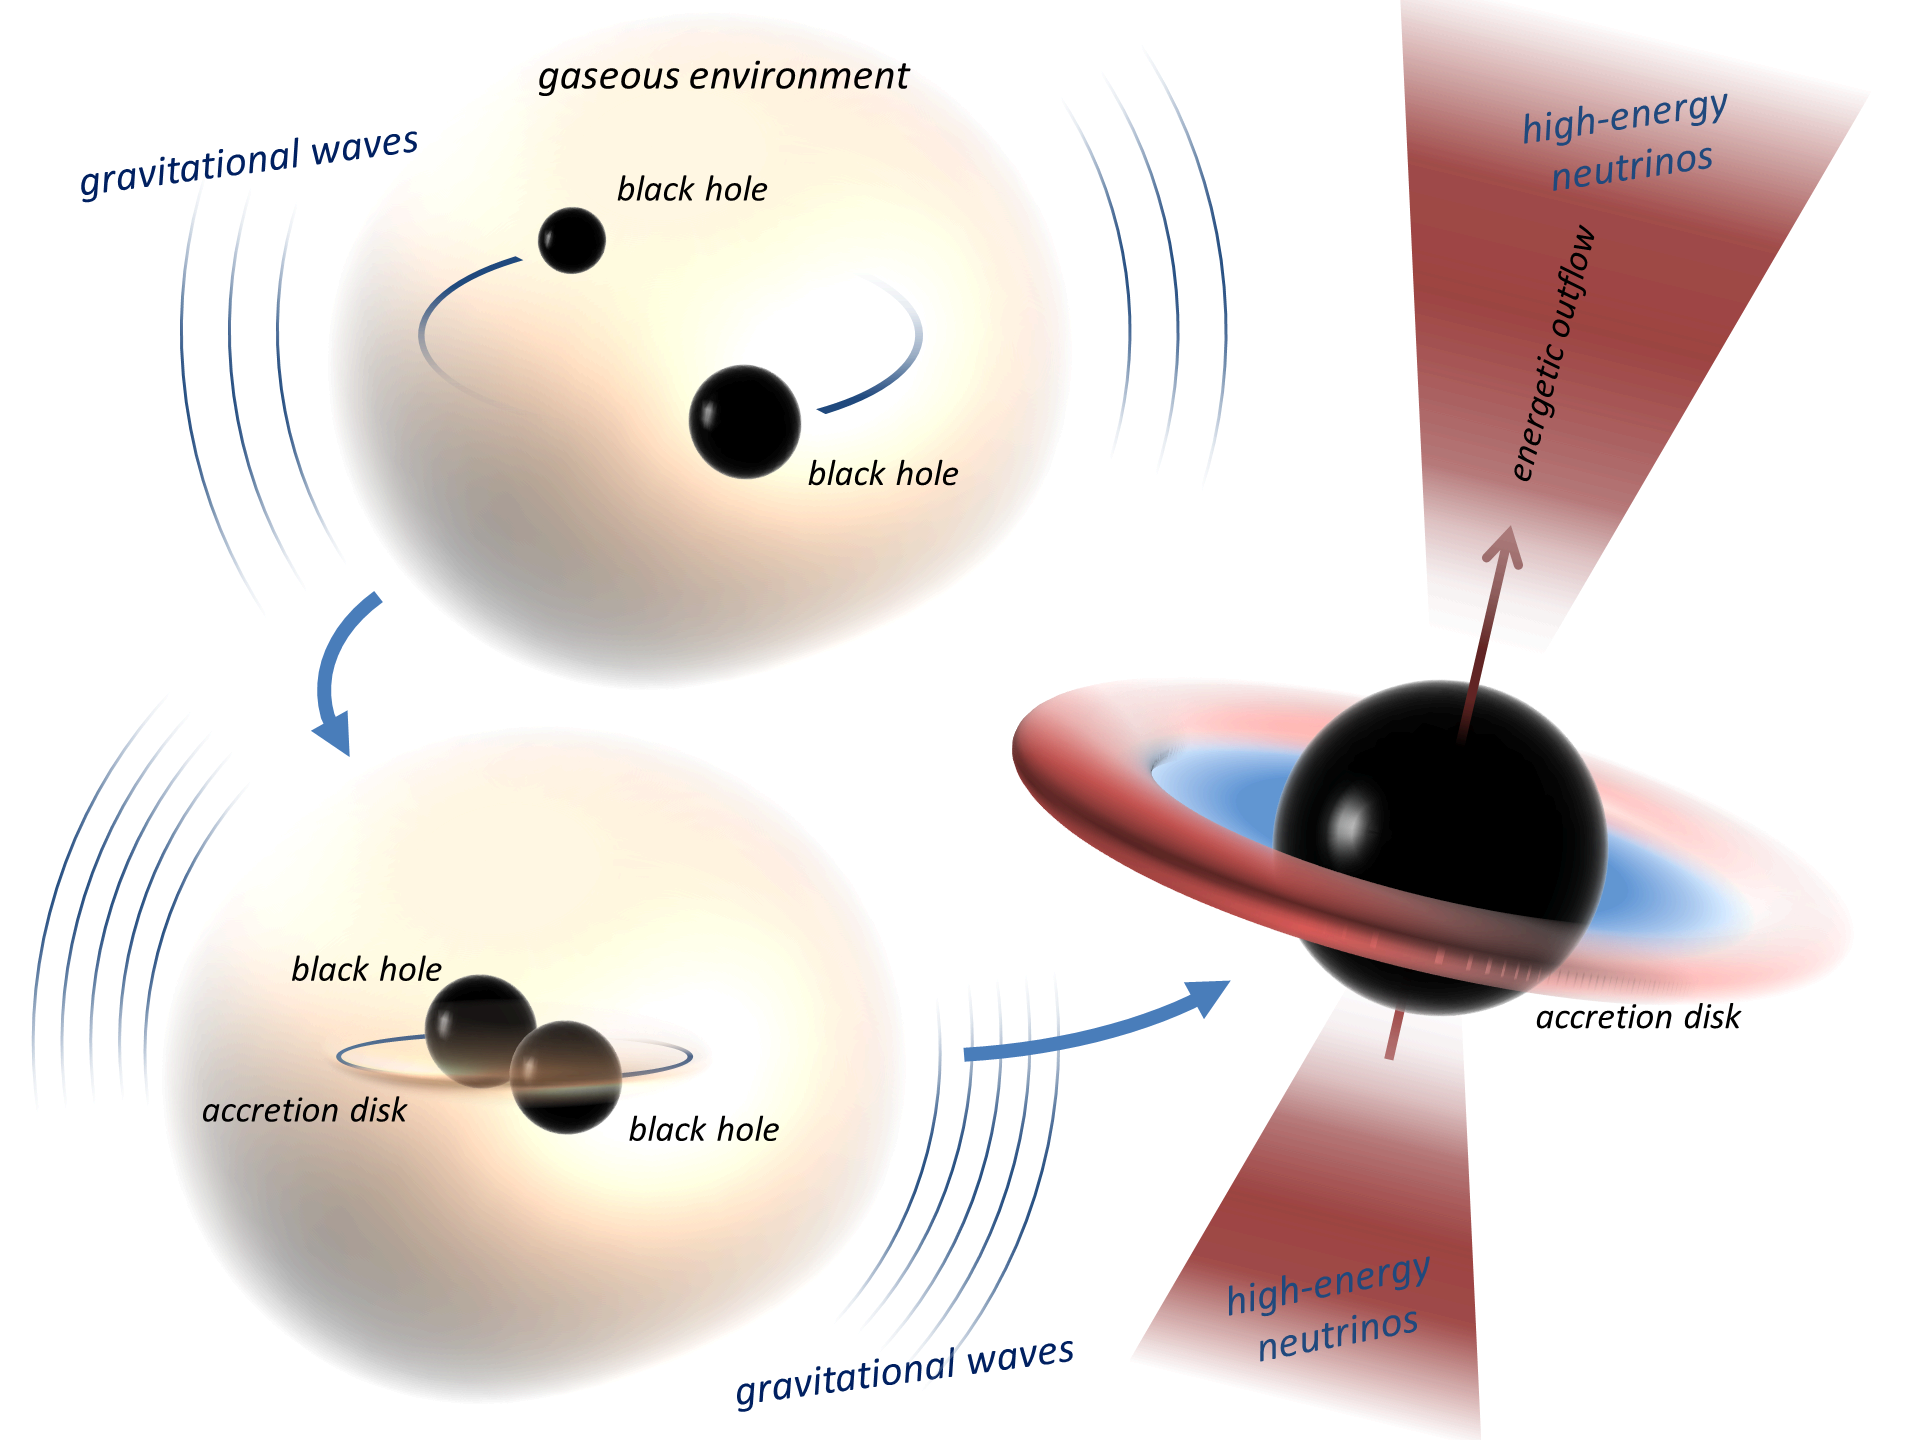
\includegraphics[width=0.5\columnwidth]{fig-bhbh-nu-64.png}
\end{center}

\ul

  \item LVC sensitive to O(Gpc)

  \item If surrounded by gas, there might be a neutrino signal

  \item Neutron star/black hole mergers are similar

\lu

}

\frame{\frametitle{Neutron star/neutron star mergers}

\begin{center}
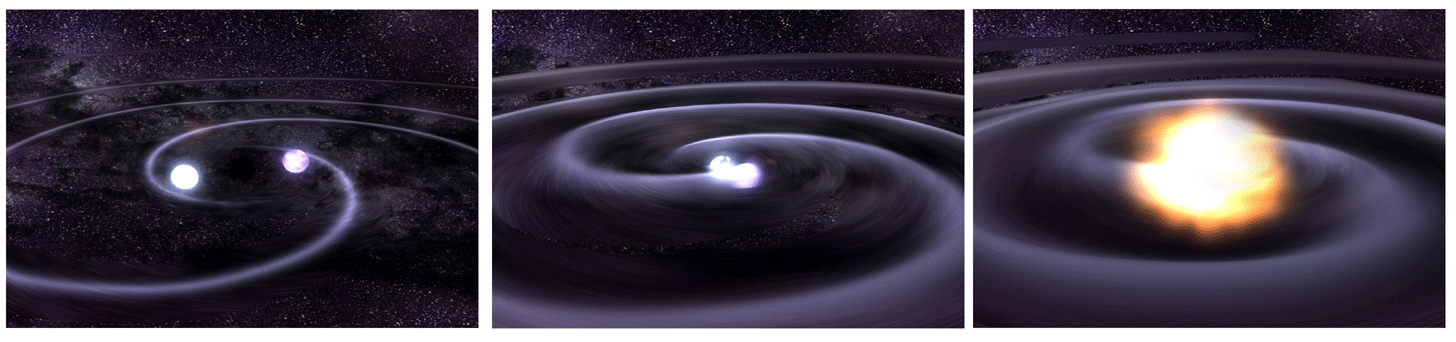
\includegraphics[width=\columnwidth]{fig-nsns-merger.jpg}
\end{center}

\ul

\item LVC sensitive to O(Gpc)

\item Similar thermal and nucleosynthesis
neutrinos to a supernova: \href{https://arxiv.org/abs/1510.06398}{arXiv:1510.06398}

  \ul

    \item Not enough to see outside the galaxy

    \item Galactic rate estimated at 0.01/century...

  \lu

\item Higher energy neutrinos from the inspiral? 
\href{http://www.sciencedirect.com/science/article/pii/S2214404816300118}{Example paper}

\lu

}

\frame{\frametitle{Supernovae}

\begin{center}
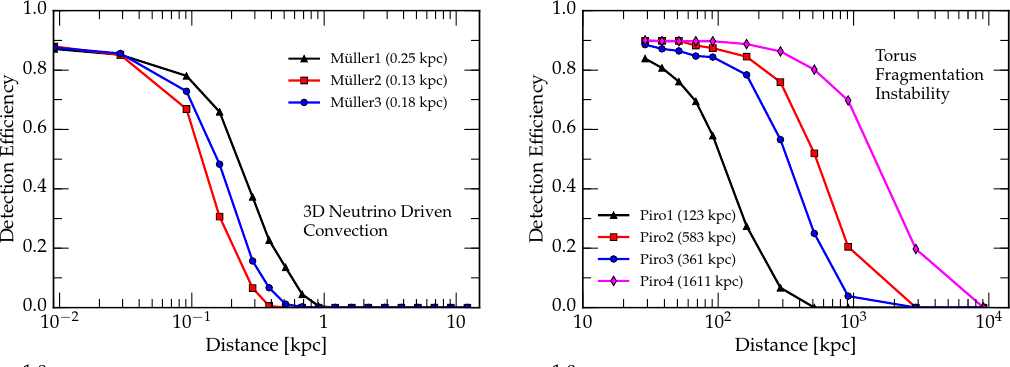
\includegraphics[width=0.8\columnwidth]{fig-ligo-supernova-sensitivity.png}
\end{center}

\ul

  \item Large neutrino signal if it is in the galaxy

  \item LIGO reach very poorly understood (\href{https://arxiv.org/abs/1605.01785}{1605.01785})
  
  \item Model range: 130\,pc (Betelgeuse, maybe) to 740\,kpc (reaches Andromeda)

  \item The paper is rather guarded, but lower end sounds more likely

  \item Anyway, it's an independent SNEWS-like warning, maybe

\lu

}

\frame{\frametitle{Misc unknown}

\cols

\colw{0.6}

\ul

  \item LIGO does a generic burst search

  \item ``Every time humans have looked at the universe with a new set of `eyes' [\dots] they have found things that were unexpected''
  
  \item Could find something:
  \ul

    \item Relatively mundane:
      $\hcancel{whatever makes gamma ray bursts}$,
      stellar-mass star mergers

    \item Exotic, but described: oscillating cosmic strings (\href{https://arxiv.org/abs/0904.4718}{0904.4718}), domain walls
    \item Something totally unanticipated
  \lu

\lu

\colbrw{0.4}

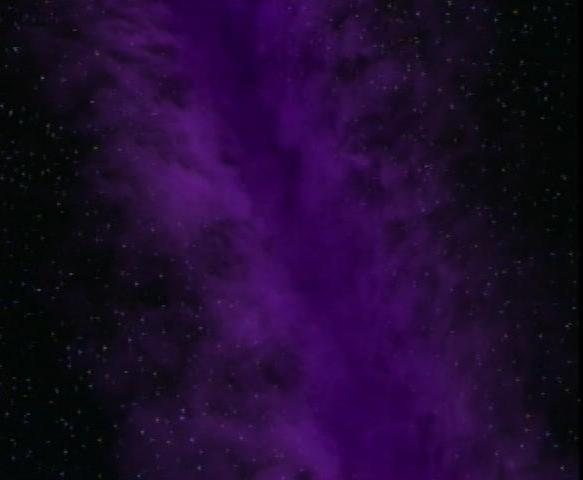
\includegraphics[width=\columnwidth]{fig-star-trek-cosmic-string.jpg}

\sloc

}

\frame{\frametitle{Analysis Outline}

\ul

\item For each GW event, use the triggers that we had running
to search for anything unusual in a $\{-500, +500\}$ second window around
the event

\item Plan written up in \href{https://nova-docdb.fnal.gov/cgi-bin/private/ShowDocument?docid=22025}{doc-22025} (soon to be updated to v2)

\item Test on randomly chosen timestamps

\item When satisfied, turn it loose on the LVC events

\lu

}

\frame{\frametitle{Triggers, pt. 1}

\ul

 \item ND activity

   \ul

     \item Count triggers, tracks, contained events

     \item \alert{Ready}, except for code to select within a region of the sky (ditto for all other events with pointing)

   \lu

  \item ND BNB

    \ul

      \item Provides $\sim 0.2\%$ unbiased livetime

      \item Search for supernova-like events

      \item Mostly a dry-run for when we trigger on GW events

      \item \alert{Not ready}.  Need a Monte Carlo supernova to tune on.

    \lu

\lu

}

\frame{\frametitle{Triggers, pt. 2}

\ul

  \item FD 10\,Hz pulser

  \ul

    \item Provides 0.55\% unbiased livetime

    \item Count tracks, contained GeV-scale events, supernova-like events

    \item \alert{Ready}

  \lu

  \item Slow monopole trigger

  \ul

    \item Not for slow monopoles, but for another $\sim 0.9\%$ livetime(!)

    \item \alert{Ready} (same as above)

  \lu

\lu

}

\frame{\frametitle{Triggers, pt. 3}

\ul

  \item Upwards-going muon

  \ul

    \item Look for upward-going muons

    \item \alert{Ready}

  \lu

\lu

}

\frame{\frametitle{Triggers, pt. 4}

\ul

  \item FD Energy

  \ul

    \item Count triggers, triggers above two energy (ADC count) thresholds, and above two energy-per-unit-time thresholds

    \item \alert{Ready}

  \lu

\lu

}

\frame{
\begin{textblock*}{\paperwidth}(0mm, 8mm)
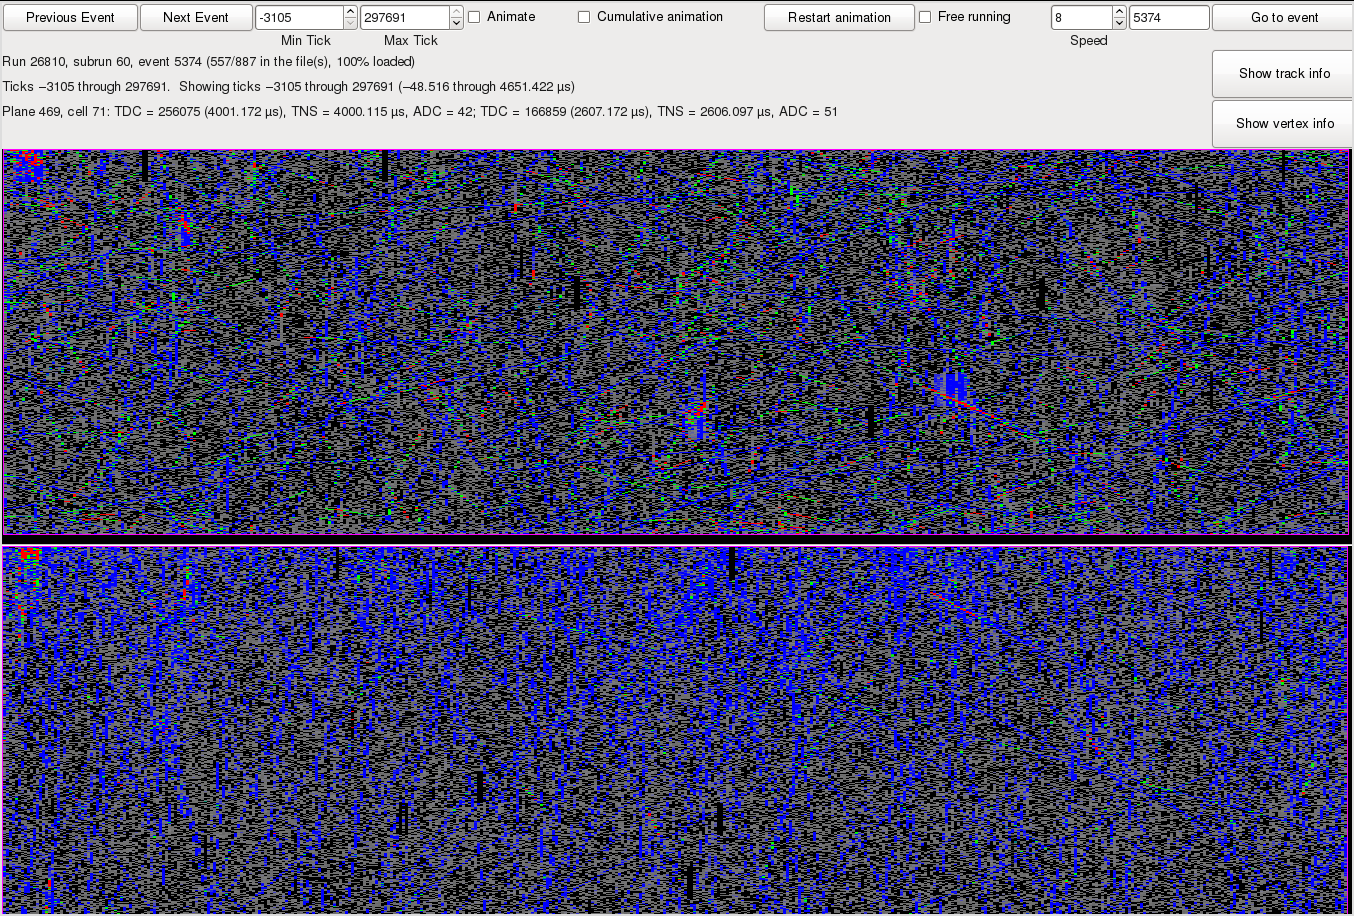
\includegraphics[width=\columnwidth]{ddenergy-40MADC-run26810-26-5374.png}
\end{textblock*}
}


\frame{
\begin{textblock*}{\paperwidth}(0mm, 8mm)
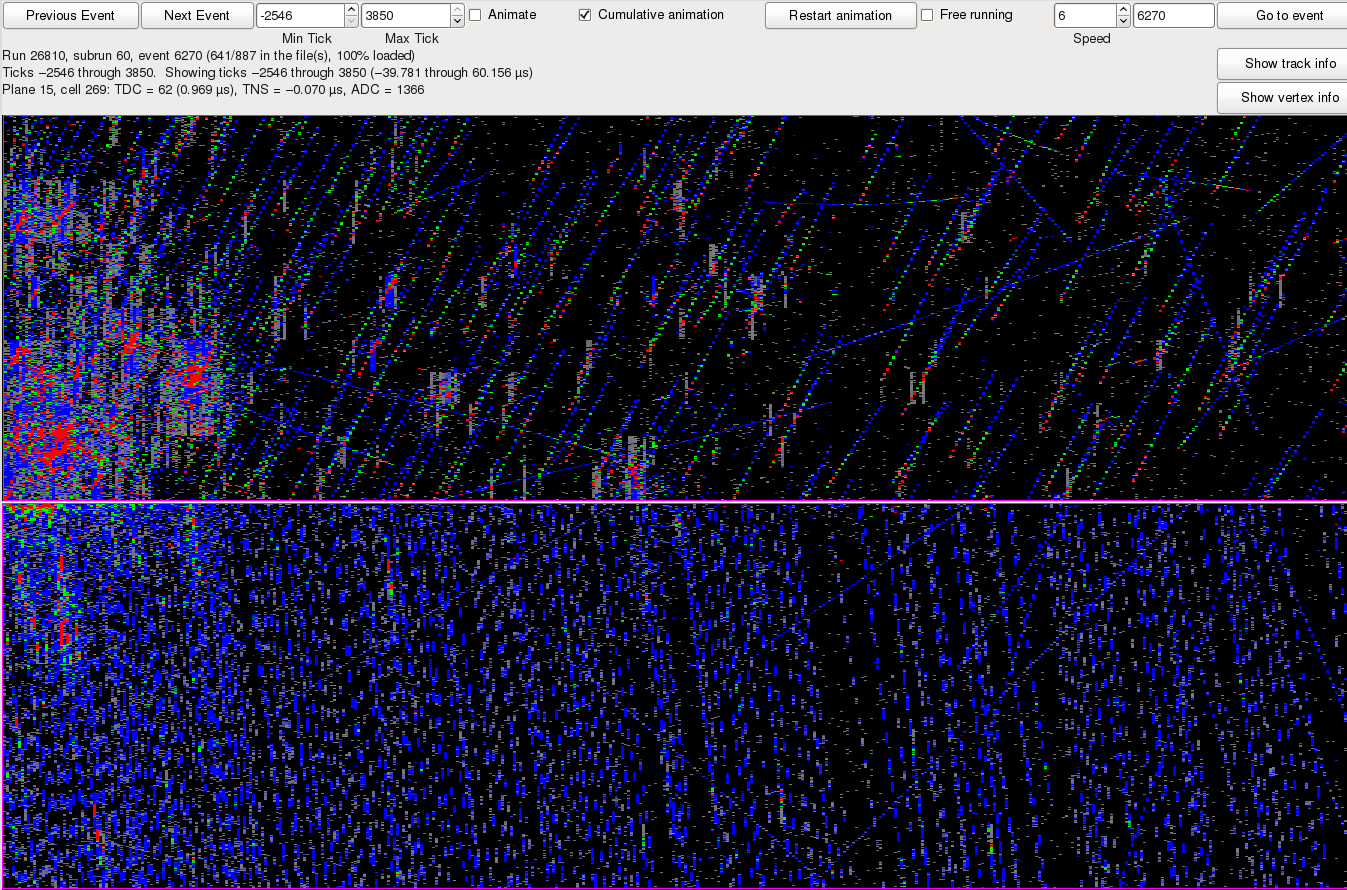
\includegraphics[width=\columnwidth]{ddenergy-3e11ADCpers-run26810-26-6270.png}
\end{textblock*}
}

\frame{
\begin{textblock*}{\paperwidth}(0mm, 8mm)
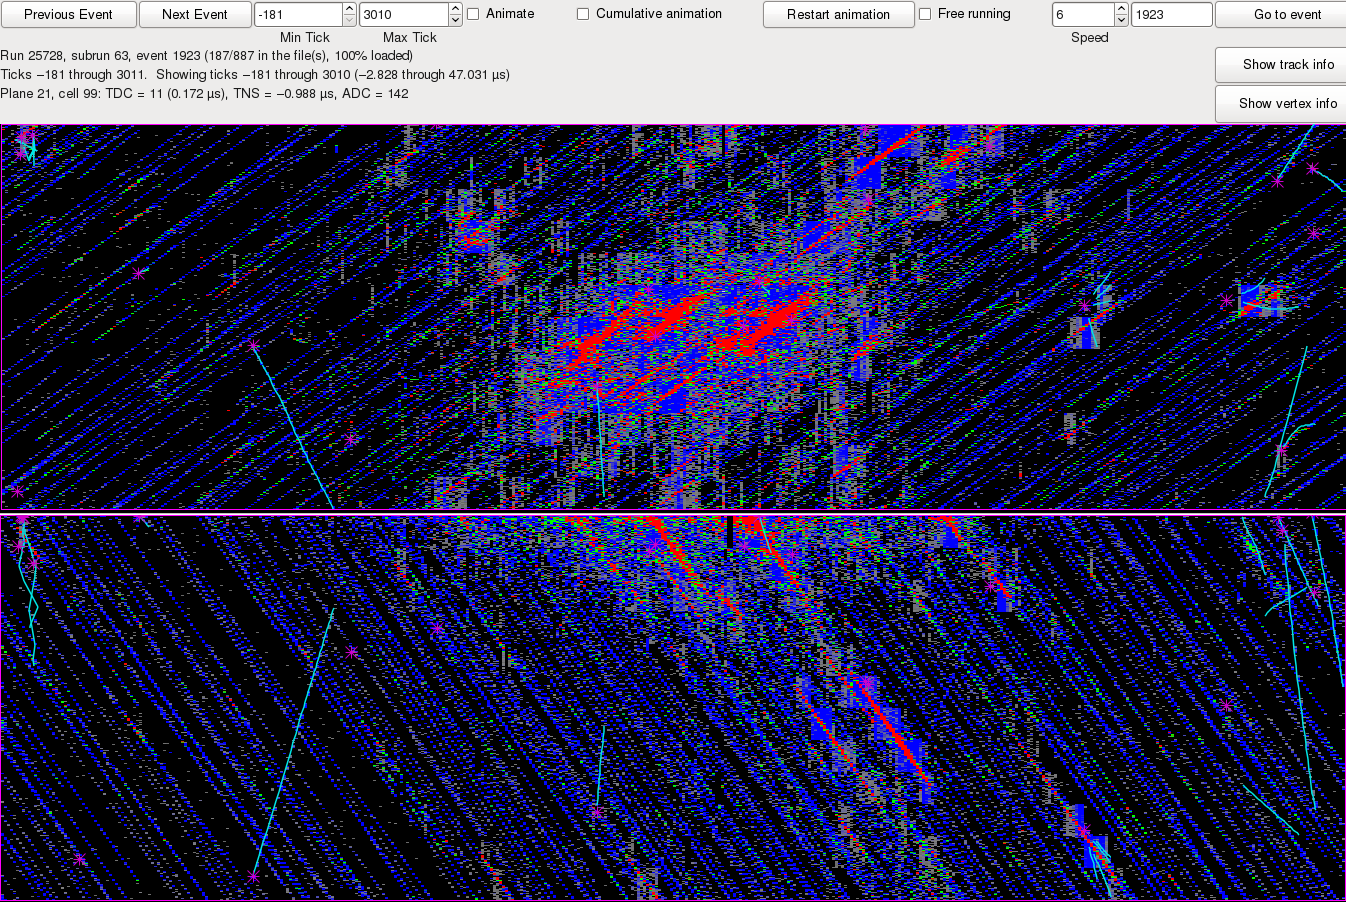
\includegraphics[width=\columnwidth]{ddenergy-9e11ADCpers-run25728-63-1923.png}
\end{textblock*}
}

\frame{\frametitle{Triggers, pt. 5}

Just count triggers:

\ul

  \item FD Contained vertex
  \item FD $\nu_\mu$
  \item FD Fast monopole

\lu


Other triggers ignored for negligible livetime and/or non-useful acceptance

\ul

\item Would use DDsupernova if available, of course!

\lu

}

\frame{\frametitle{Rationale}

\ul

\item This is largely an exercise to prepare for future events

\item Tiny livetimes mean no chance of seeing a low-energy burst, especially 
since Super-K, Borexino and KamLAND have already reported null results

  \ul

  \item In the future, we can trigger on LIGO/VIRGO events and get 100\% livetime

  \lu

\item For triggered events, not as hopeless, but only
within phase space not excluded by Super-K and IceCube

\lu

}

\frame{\frametitle{Testing}

\ul

\item Have a set of random times for testing

\item My framework assumes nothing is reconstructed for me

\item Set of fcls that do all necessary reconstruction on a trigger-by-trigger
basis

\item \href{https://github.com/straitm/lvc-coin}{https://github.com/straitm/lvc-coin}


\lu

}

\frame{\frametitle{Far Detector pulser data}

\begin{center}

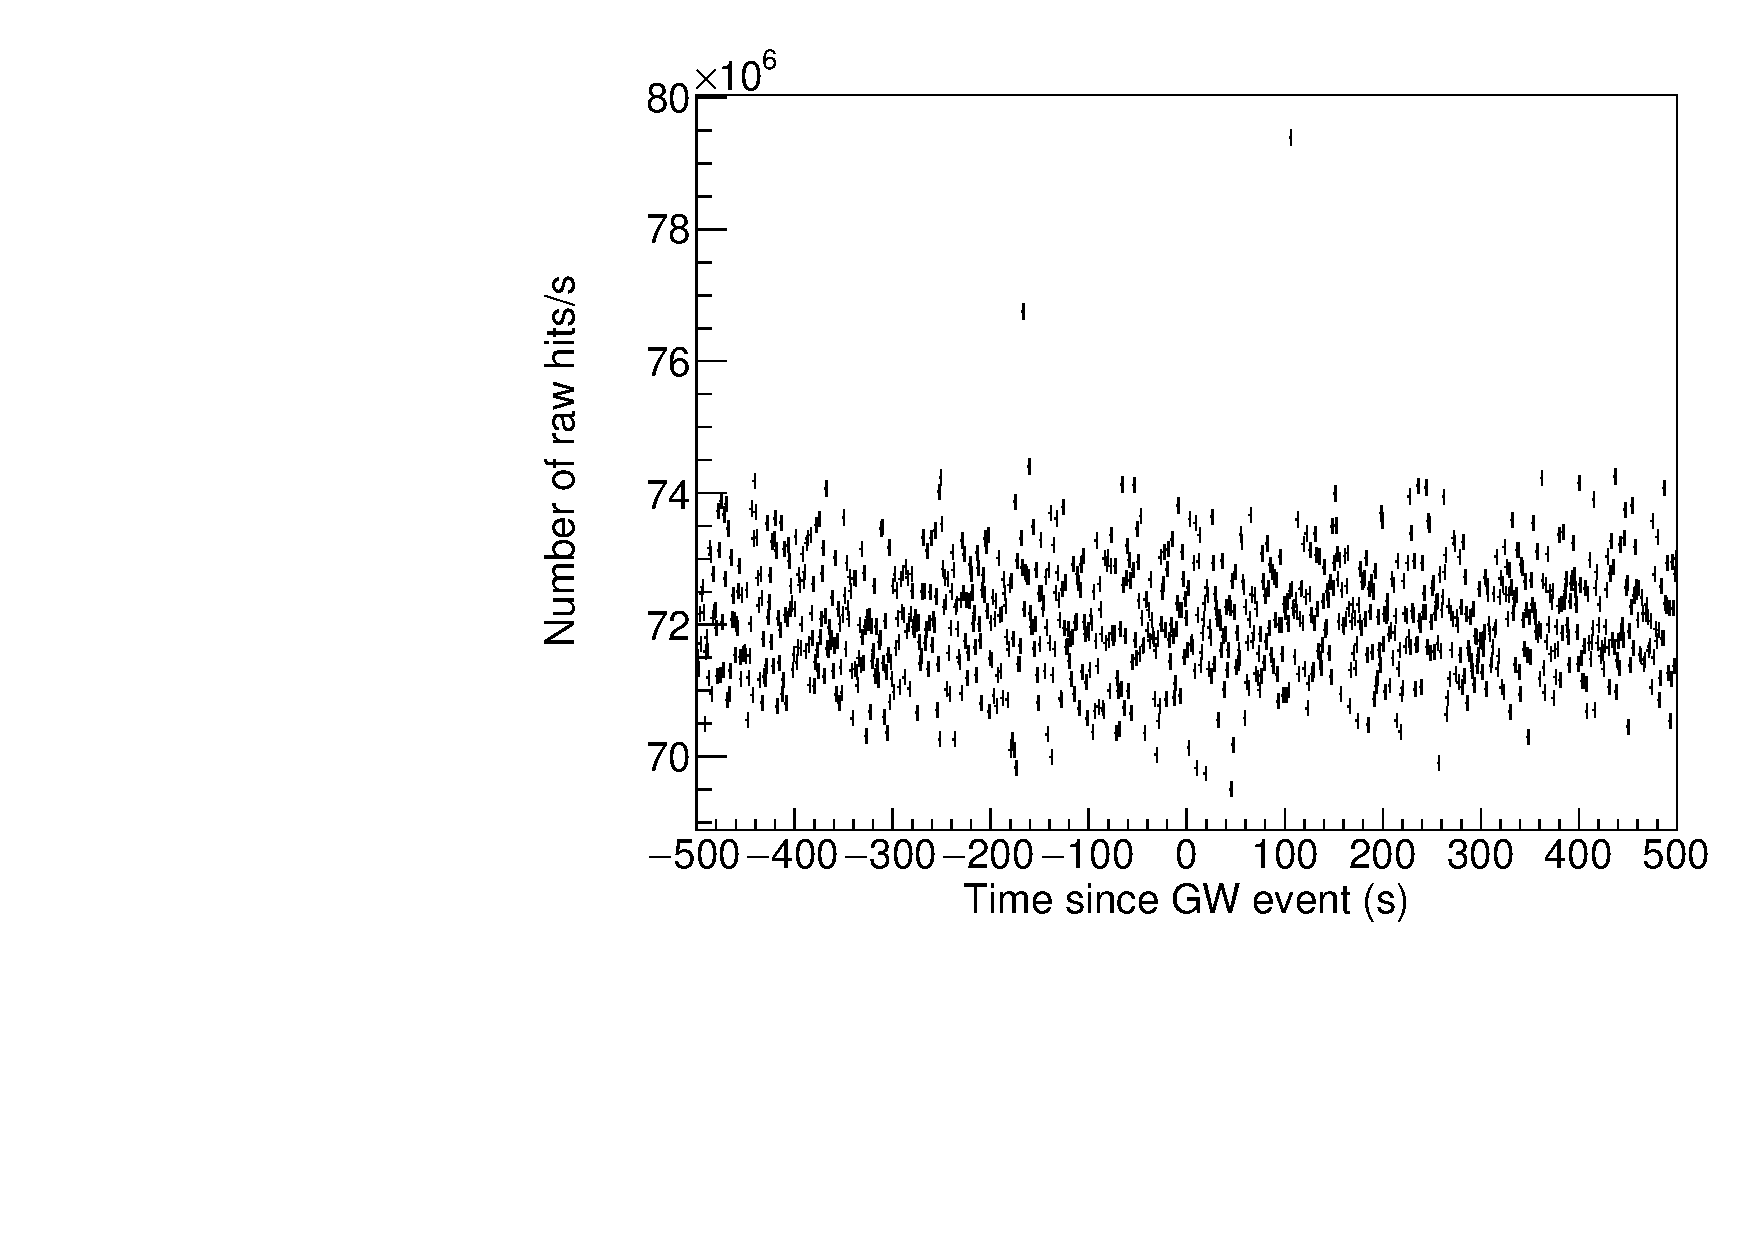
\includegraphics[width=0.333\columnwidth]{ligopass2-fardet-pulser-rawhits.pdf}%
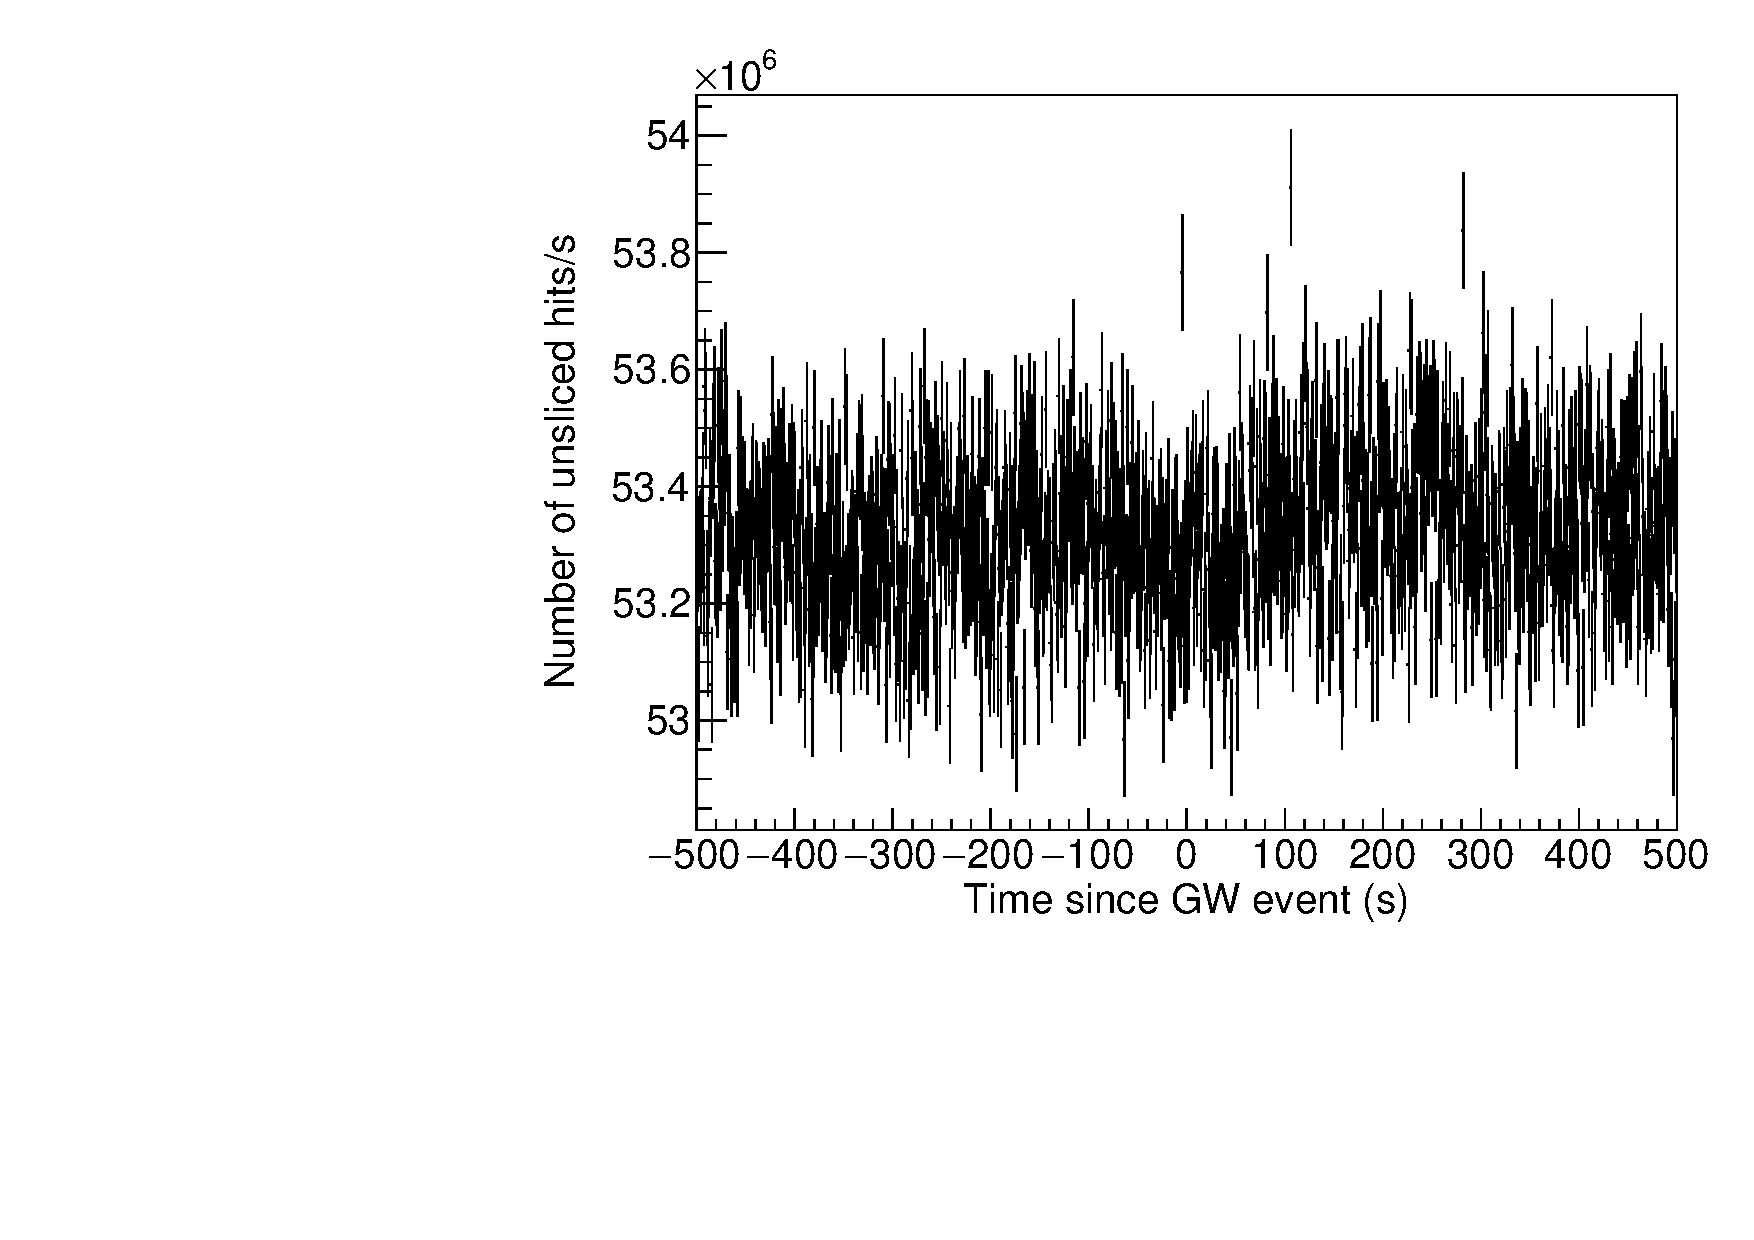
\includegraphics[width=0.333\columnwidth]{ligopass2-fardet-pulser-unslicedhits.pdf}

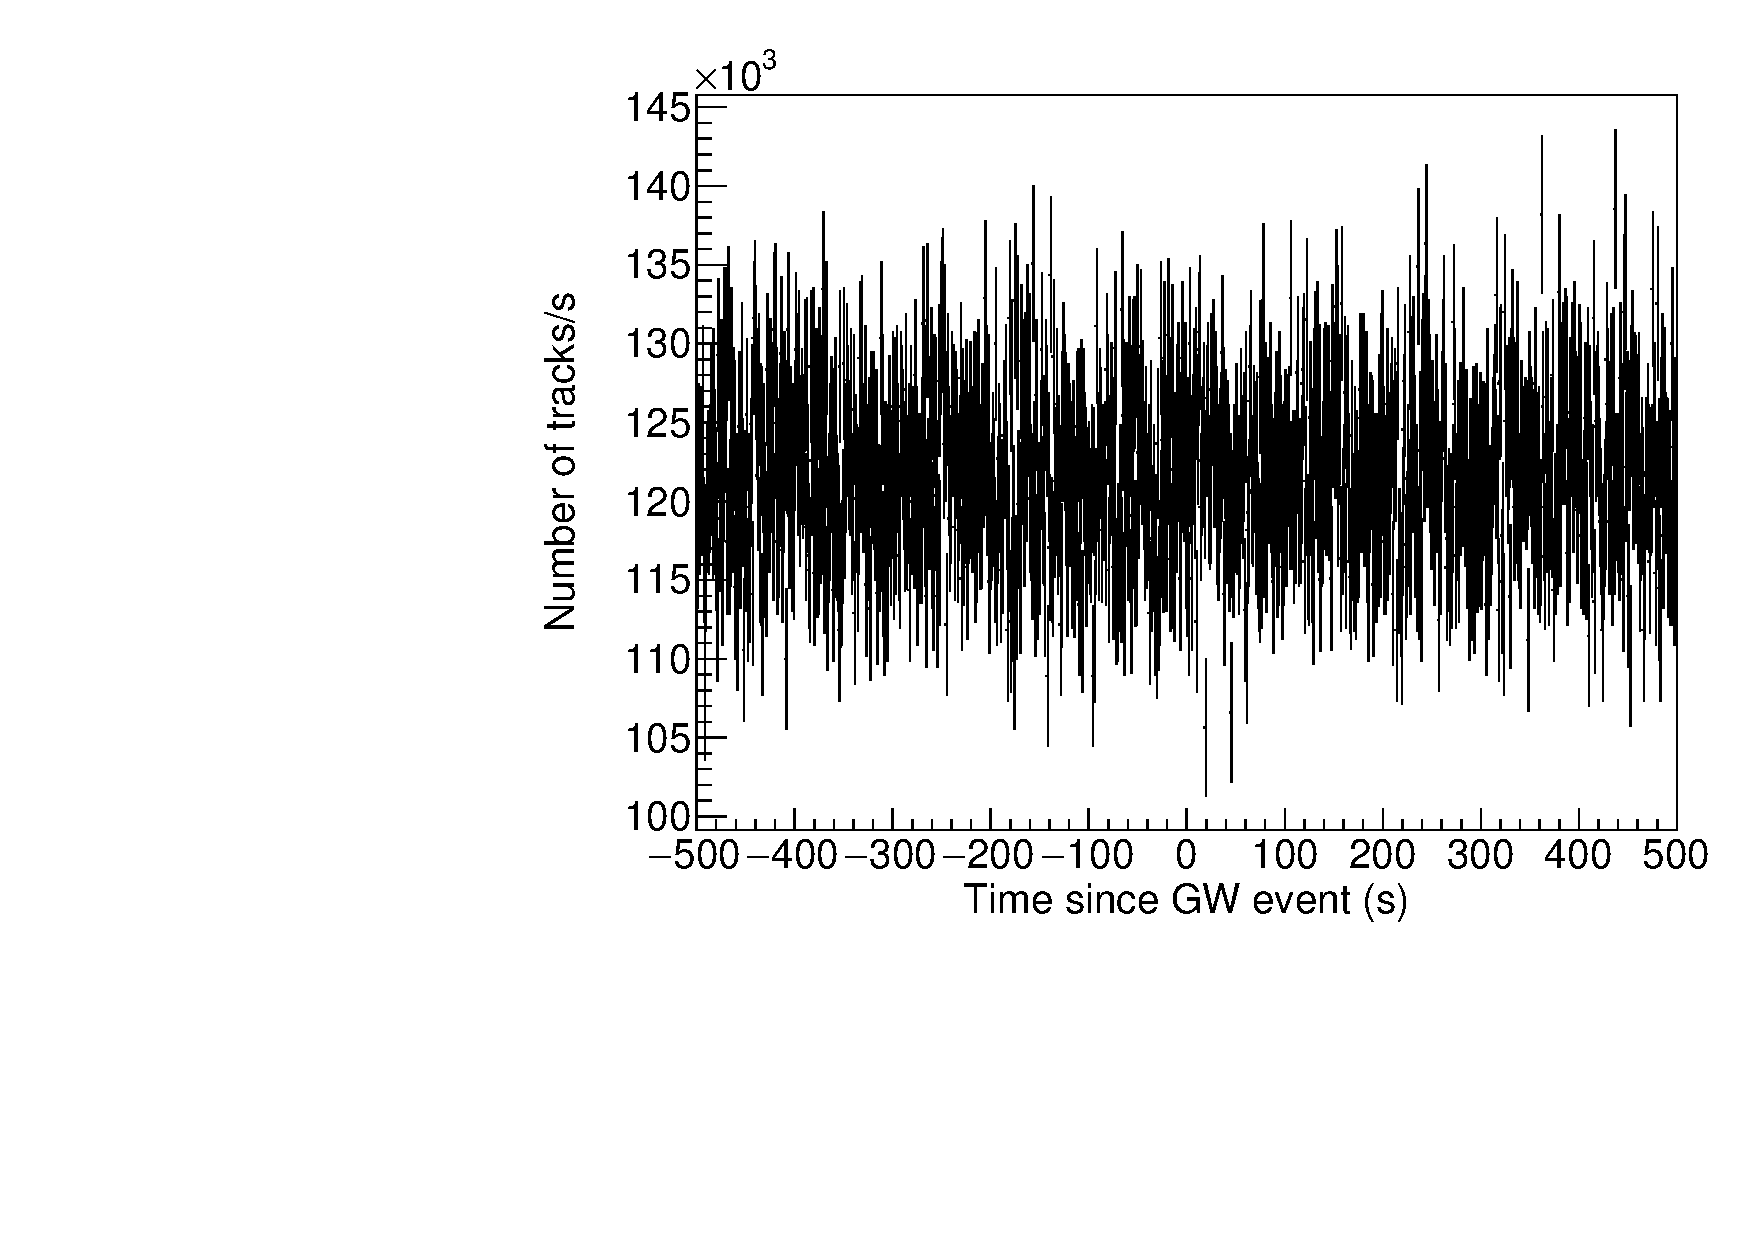
\includegraphics[width=0.333\columnwidth]{ligopass2-fardet-pulser-tracks.pdf}%
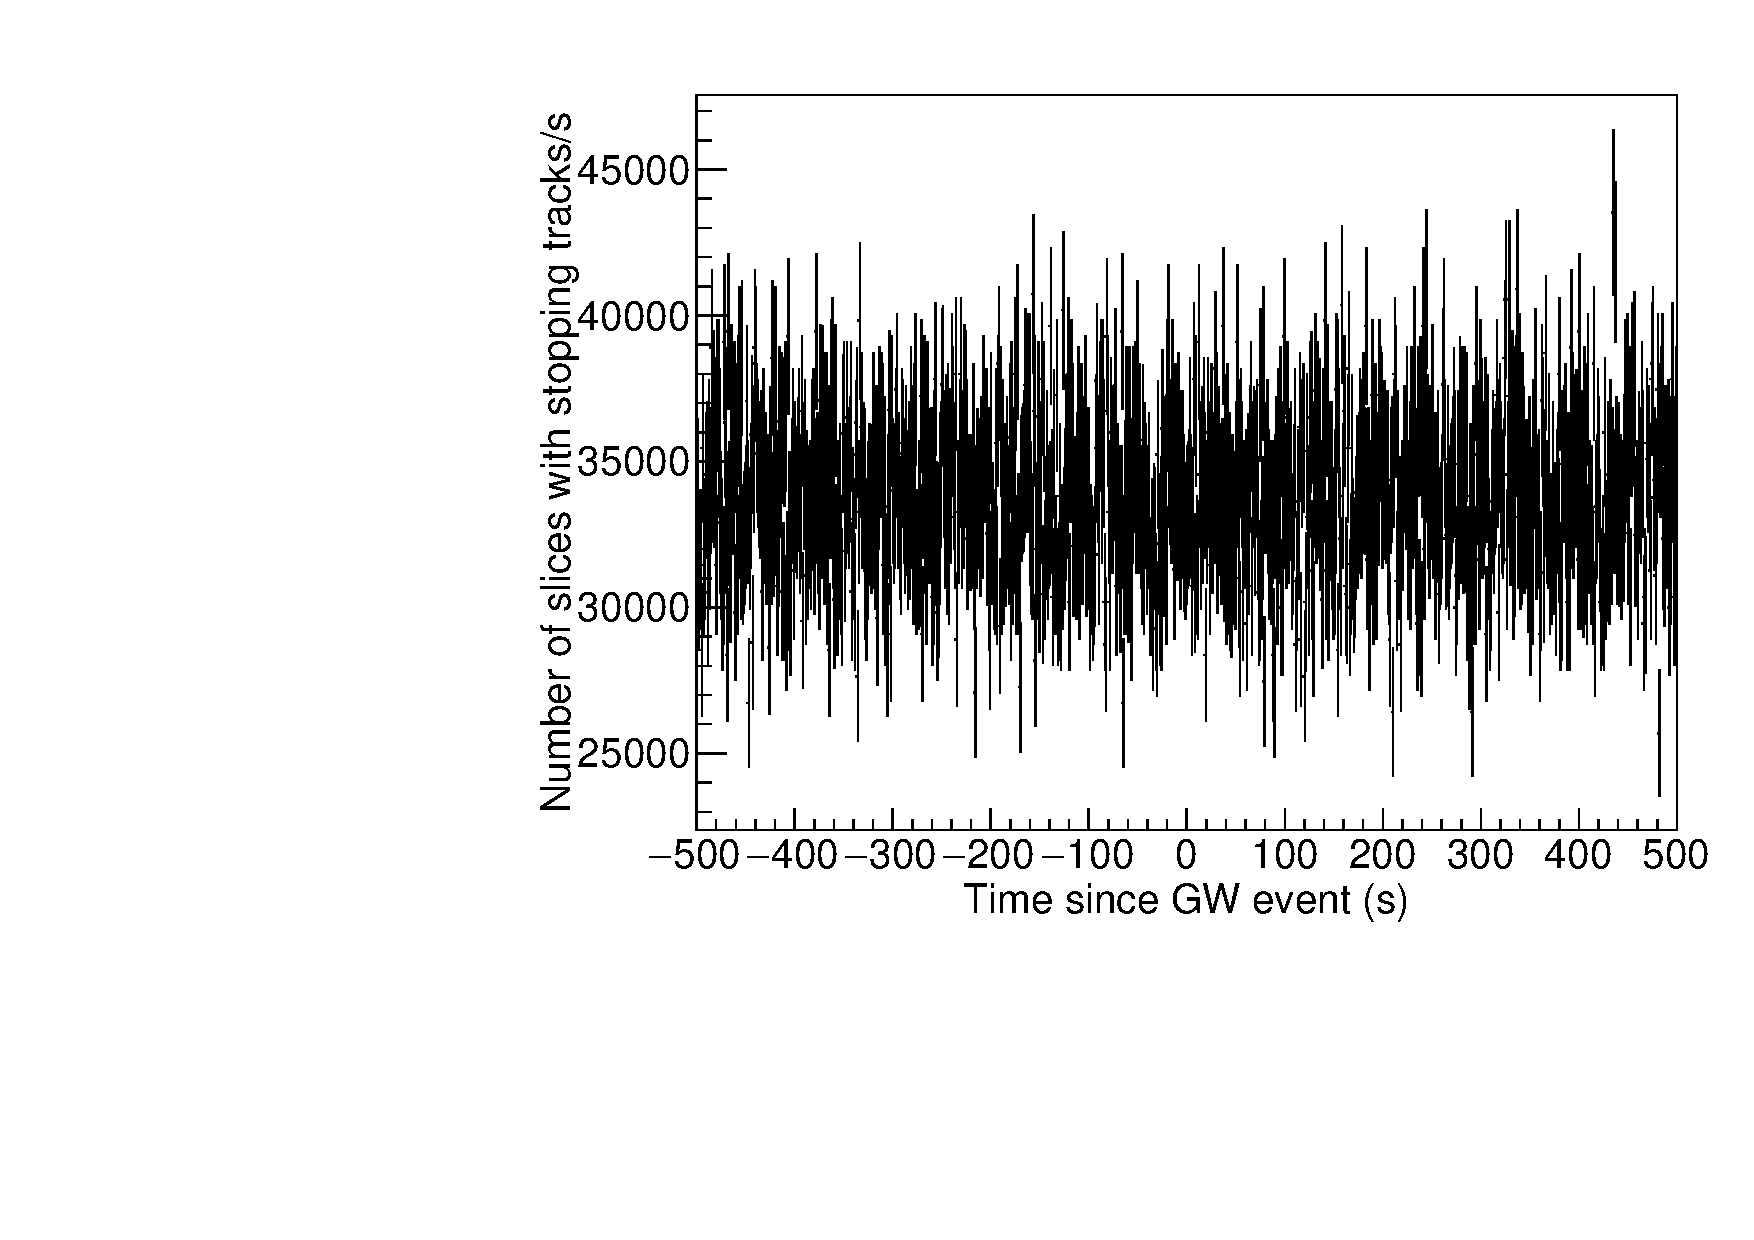
\includegraphics[width=0.333\columnwidth]{ligopass2-fardet-pulser-stoppingtracks.pdf}%
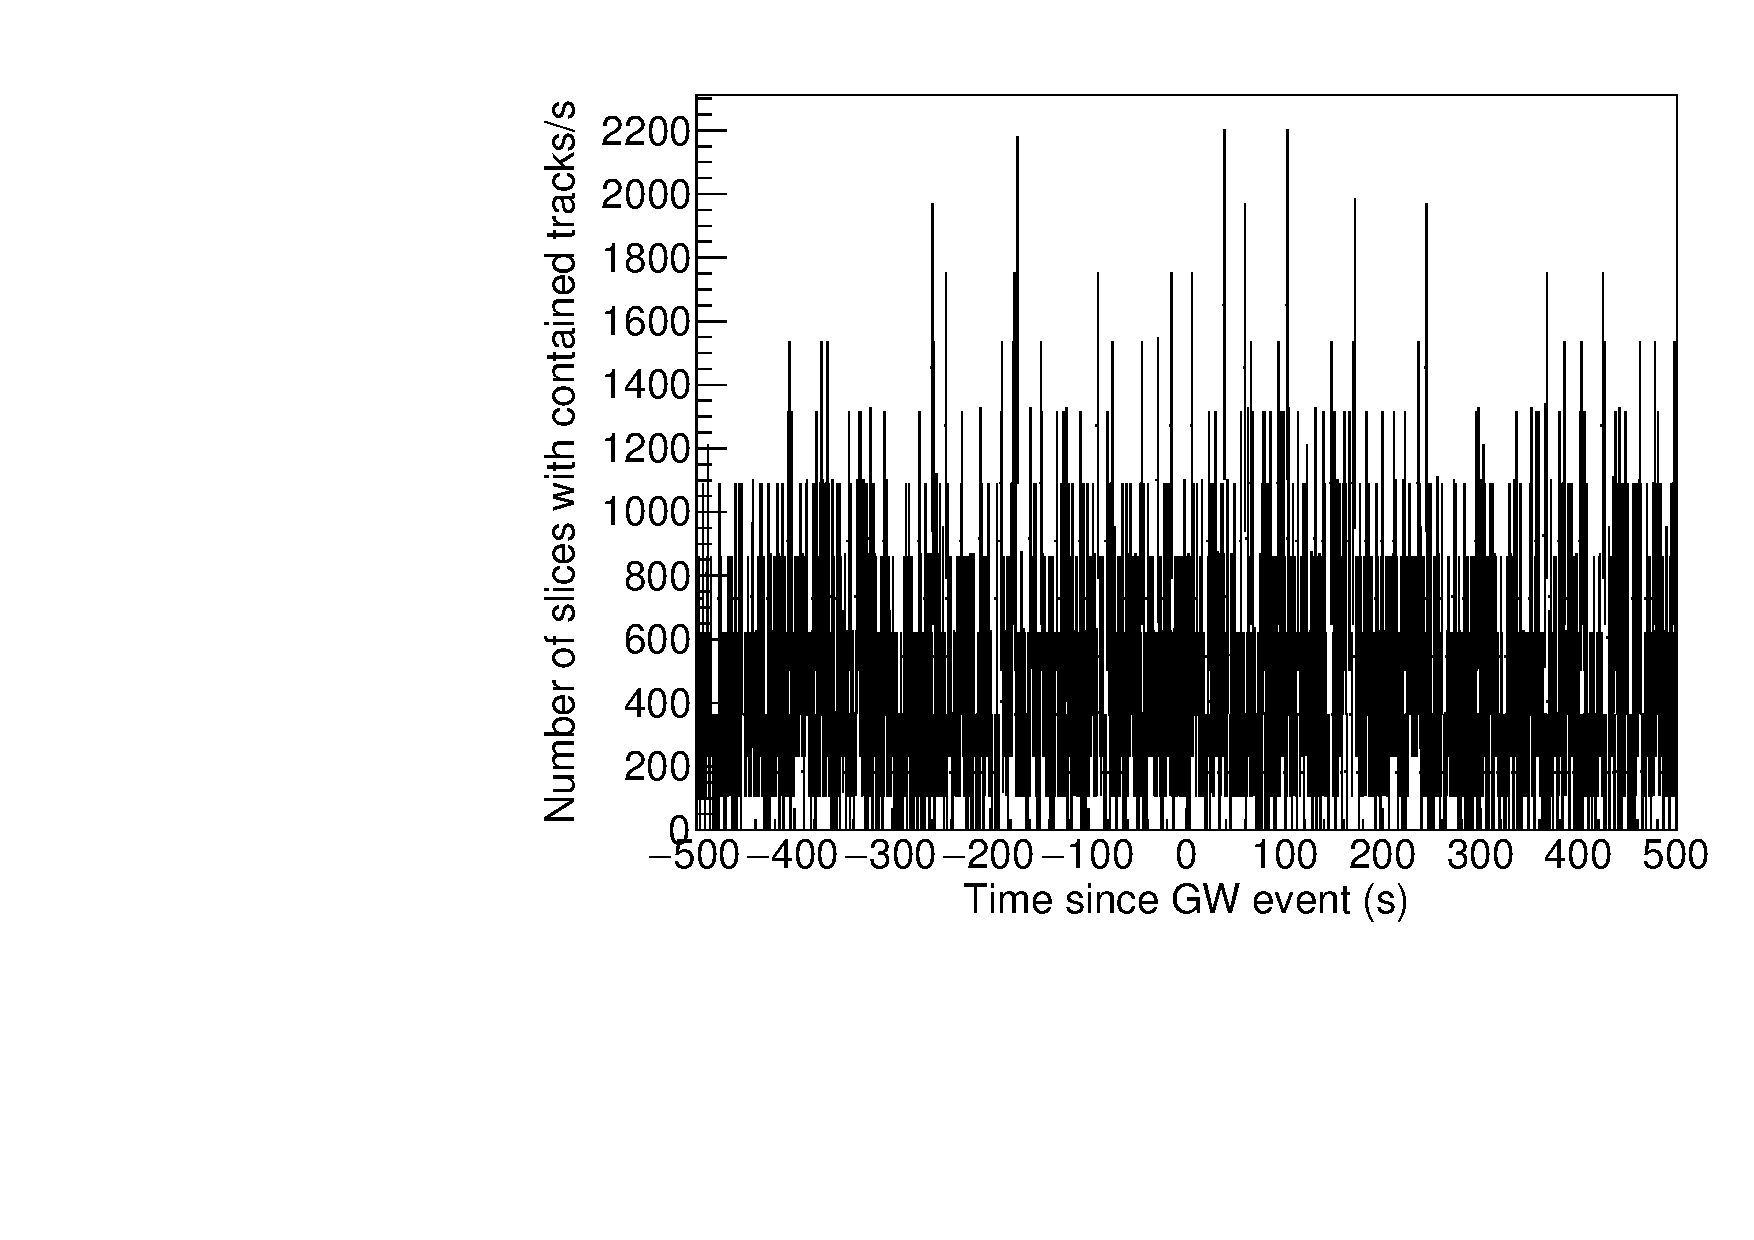
\includegraphics[width=0.333\columnwidth]{ligopass2-fardet-pulser-containedtracks.pdf}%

\end{center}

\ul

  \item .\phantom{tp}

\lu

}

\frame{\frametitle{Near Detector BNB}

\begin{center}

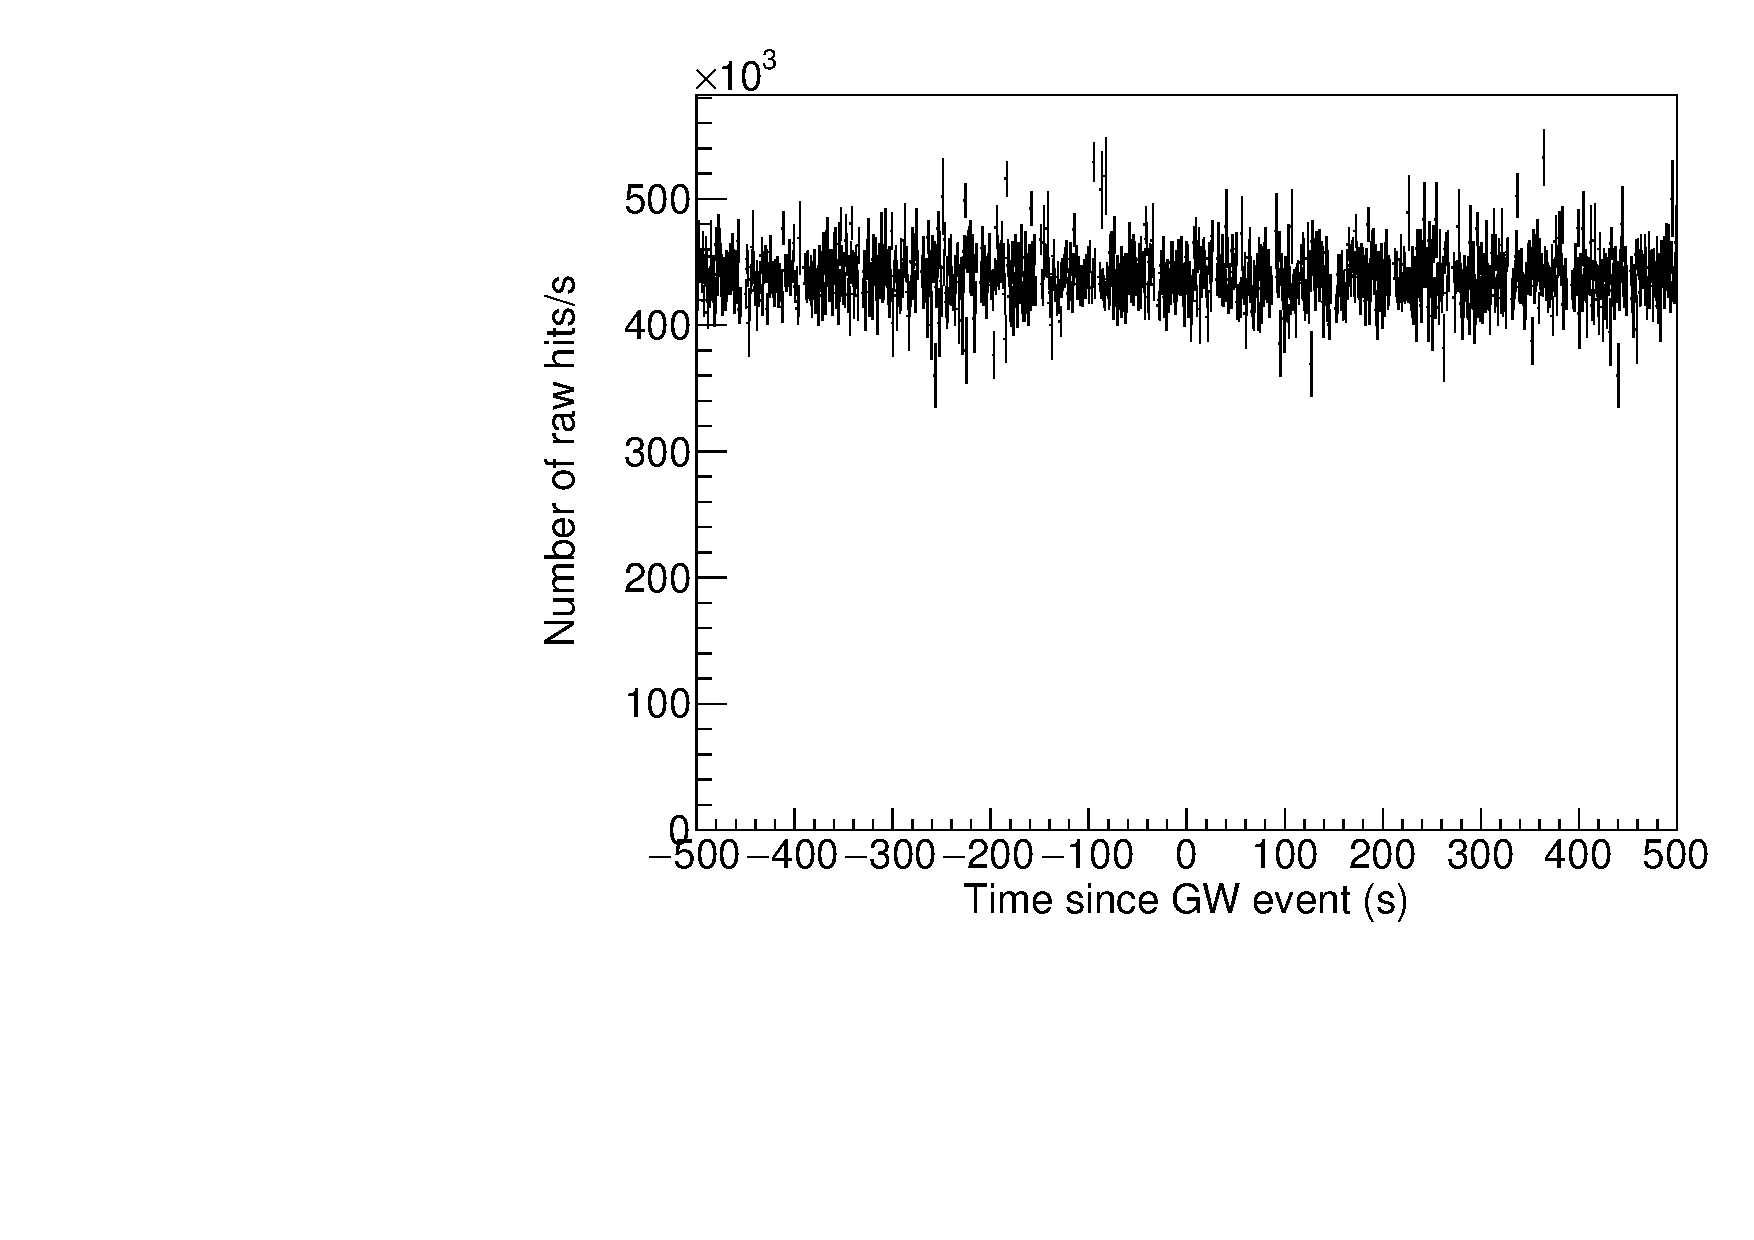
\includegraphics[width=0.333\columnwidth]{ligopass2-neardet-bnb-rawhits.pdf}%
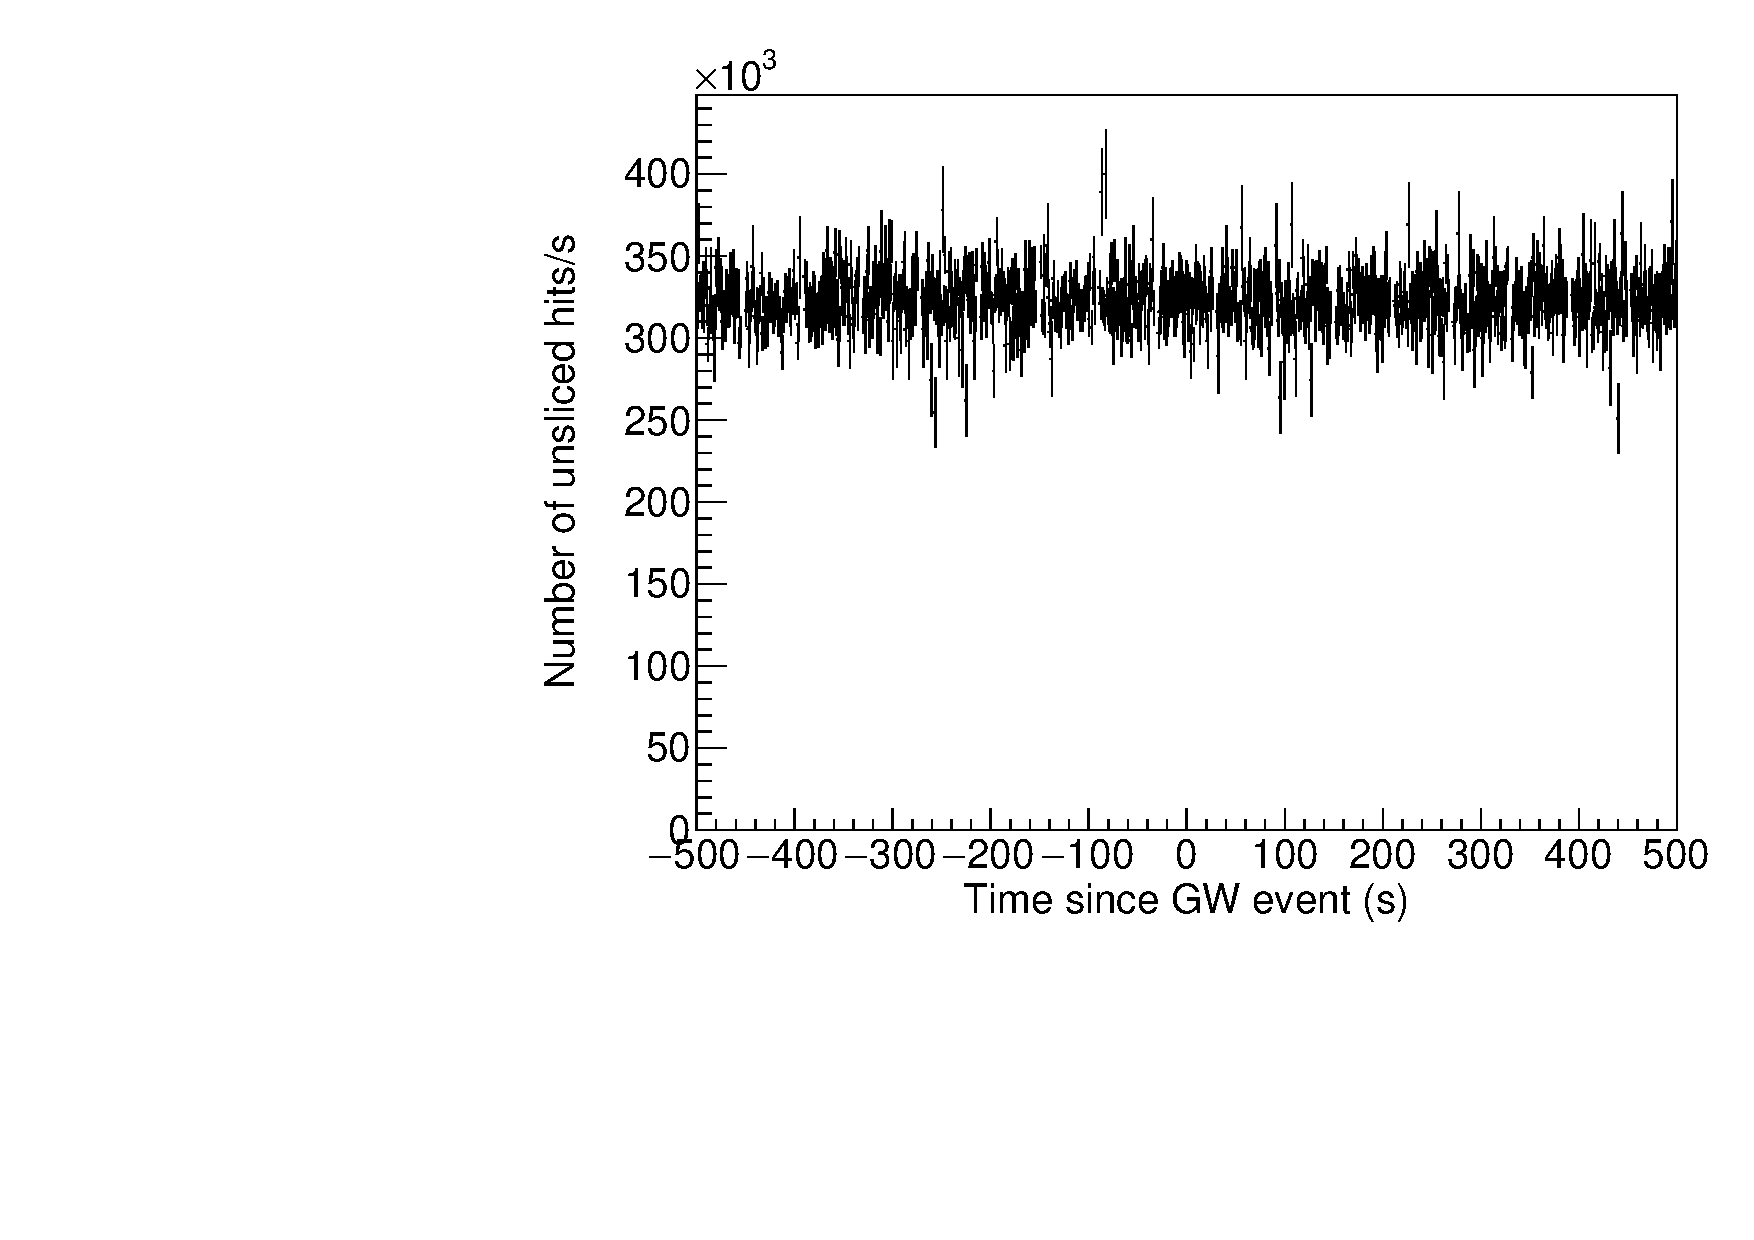
\includegraphics[width=0.333\columnwidth]{ligopass2-neardet-bnb-unslicedhits.pdf}

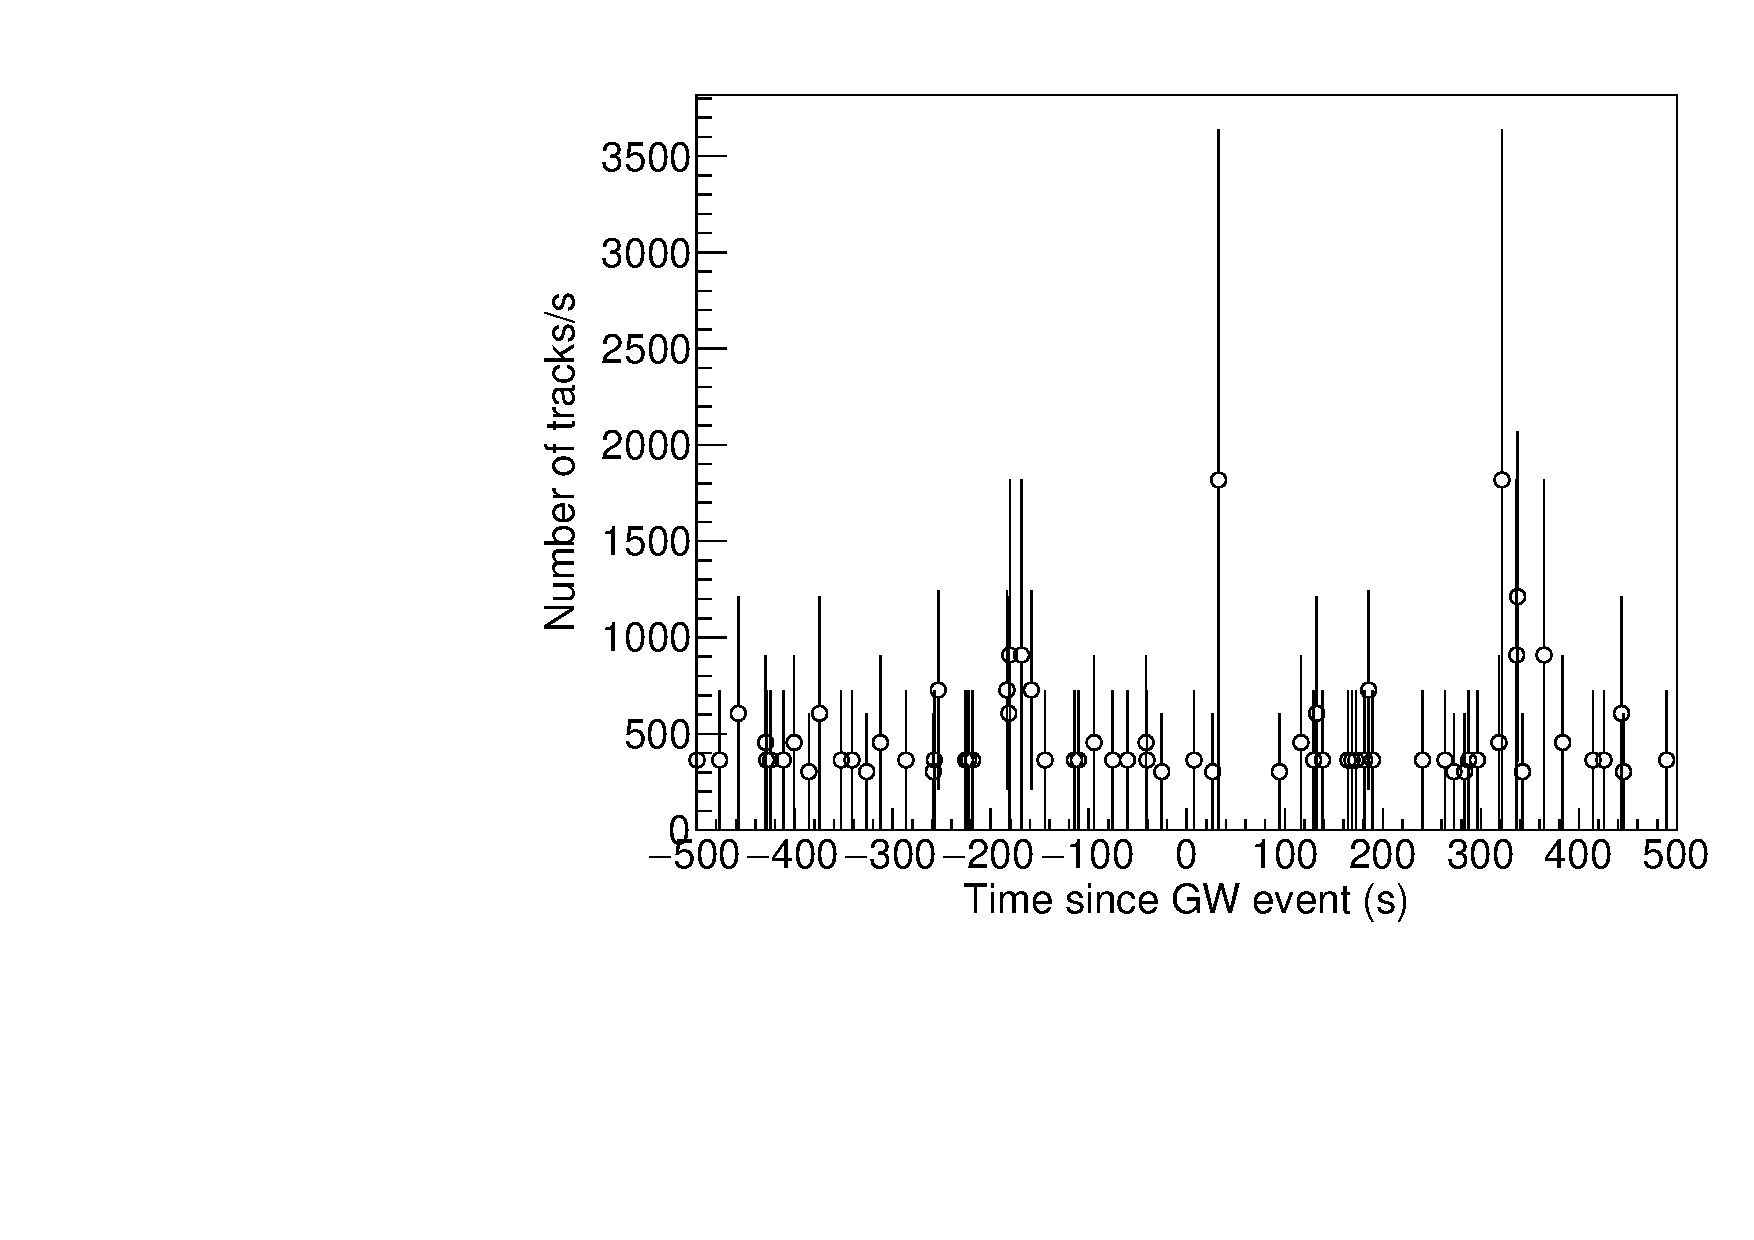
\includegraphics[width=0.333\columnwidth]{ligopass2-neardet-bnb-tracks.pdf}%
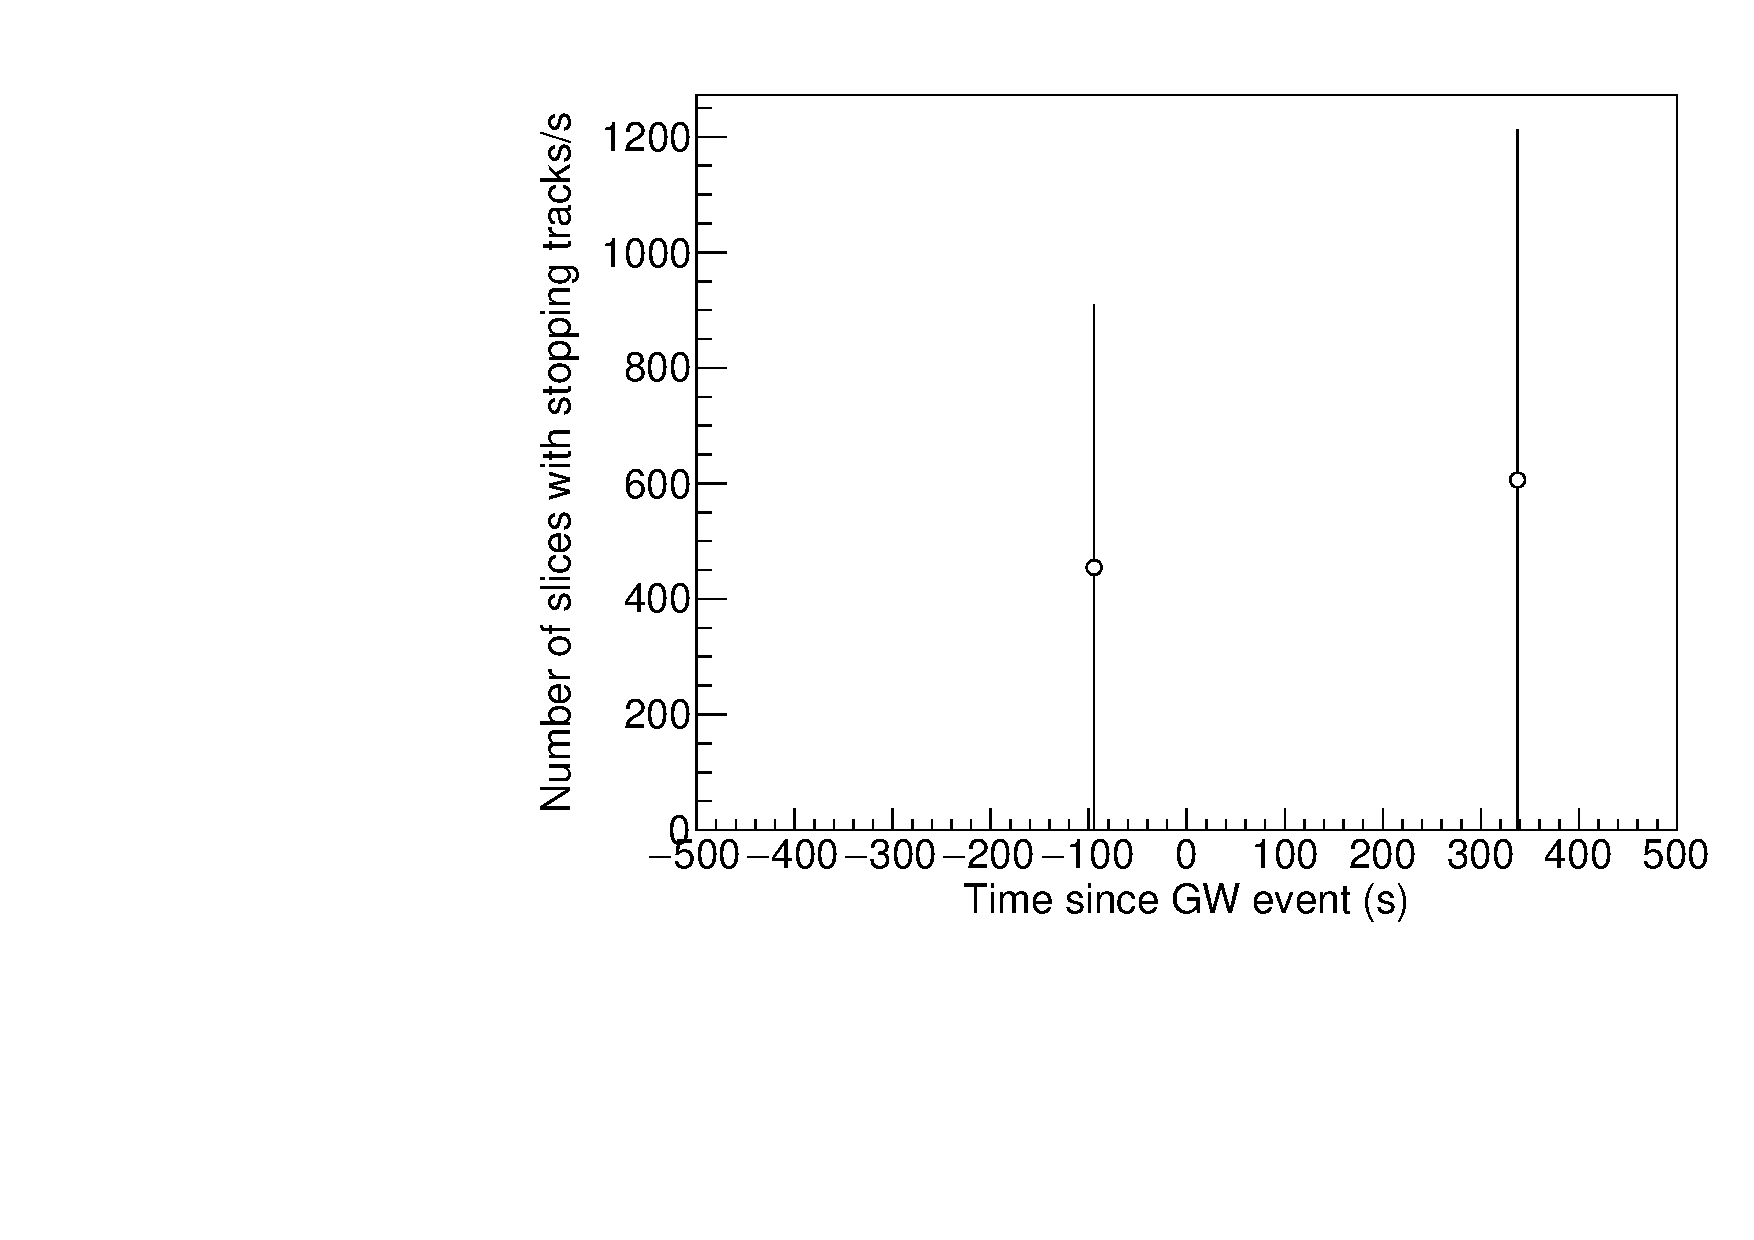
\includegraphics[width=0.333\columnwidth]{ligopass2-neardet-bnb-stoppingtracks.pdf}%
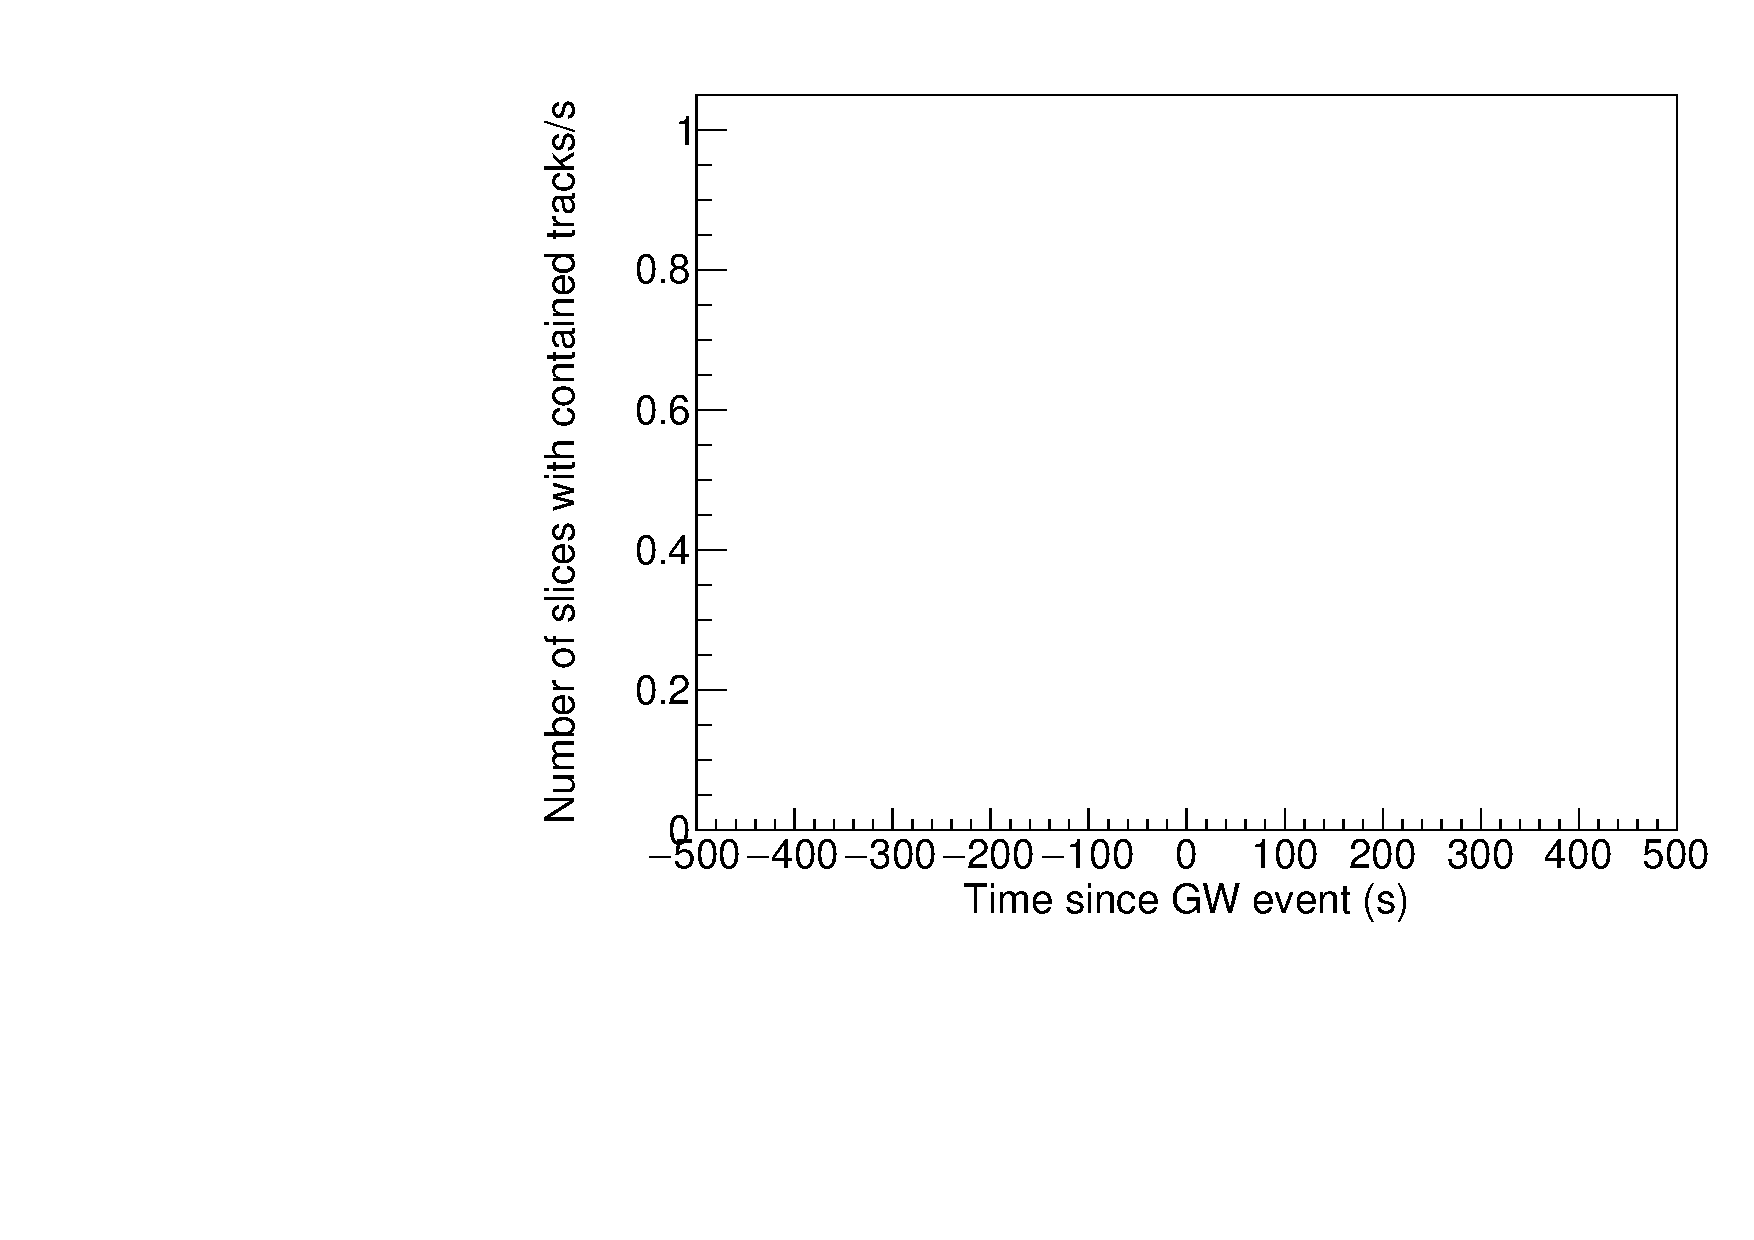
\includegraphics[width=0.333\columnwidth]{ligopass2-neardet-bnb-containedtracks.pdf}%

\end{center}

\ul

  \item BNB livetime isn't very consistent, at least around the test time

\lu

}

\frame{\frametitle{Near Detector ddactivity}

\begin{center}

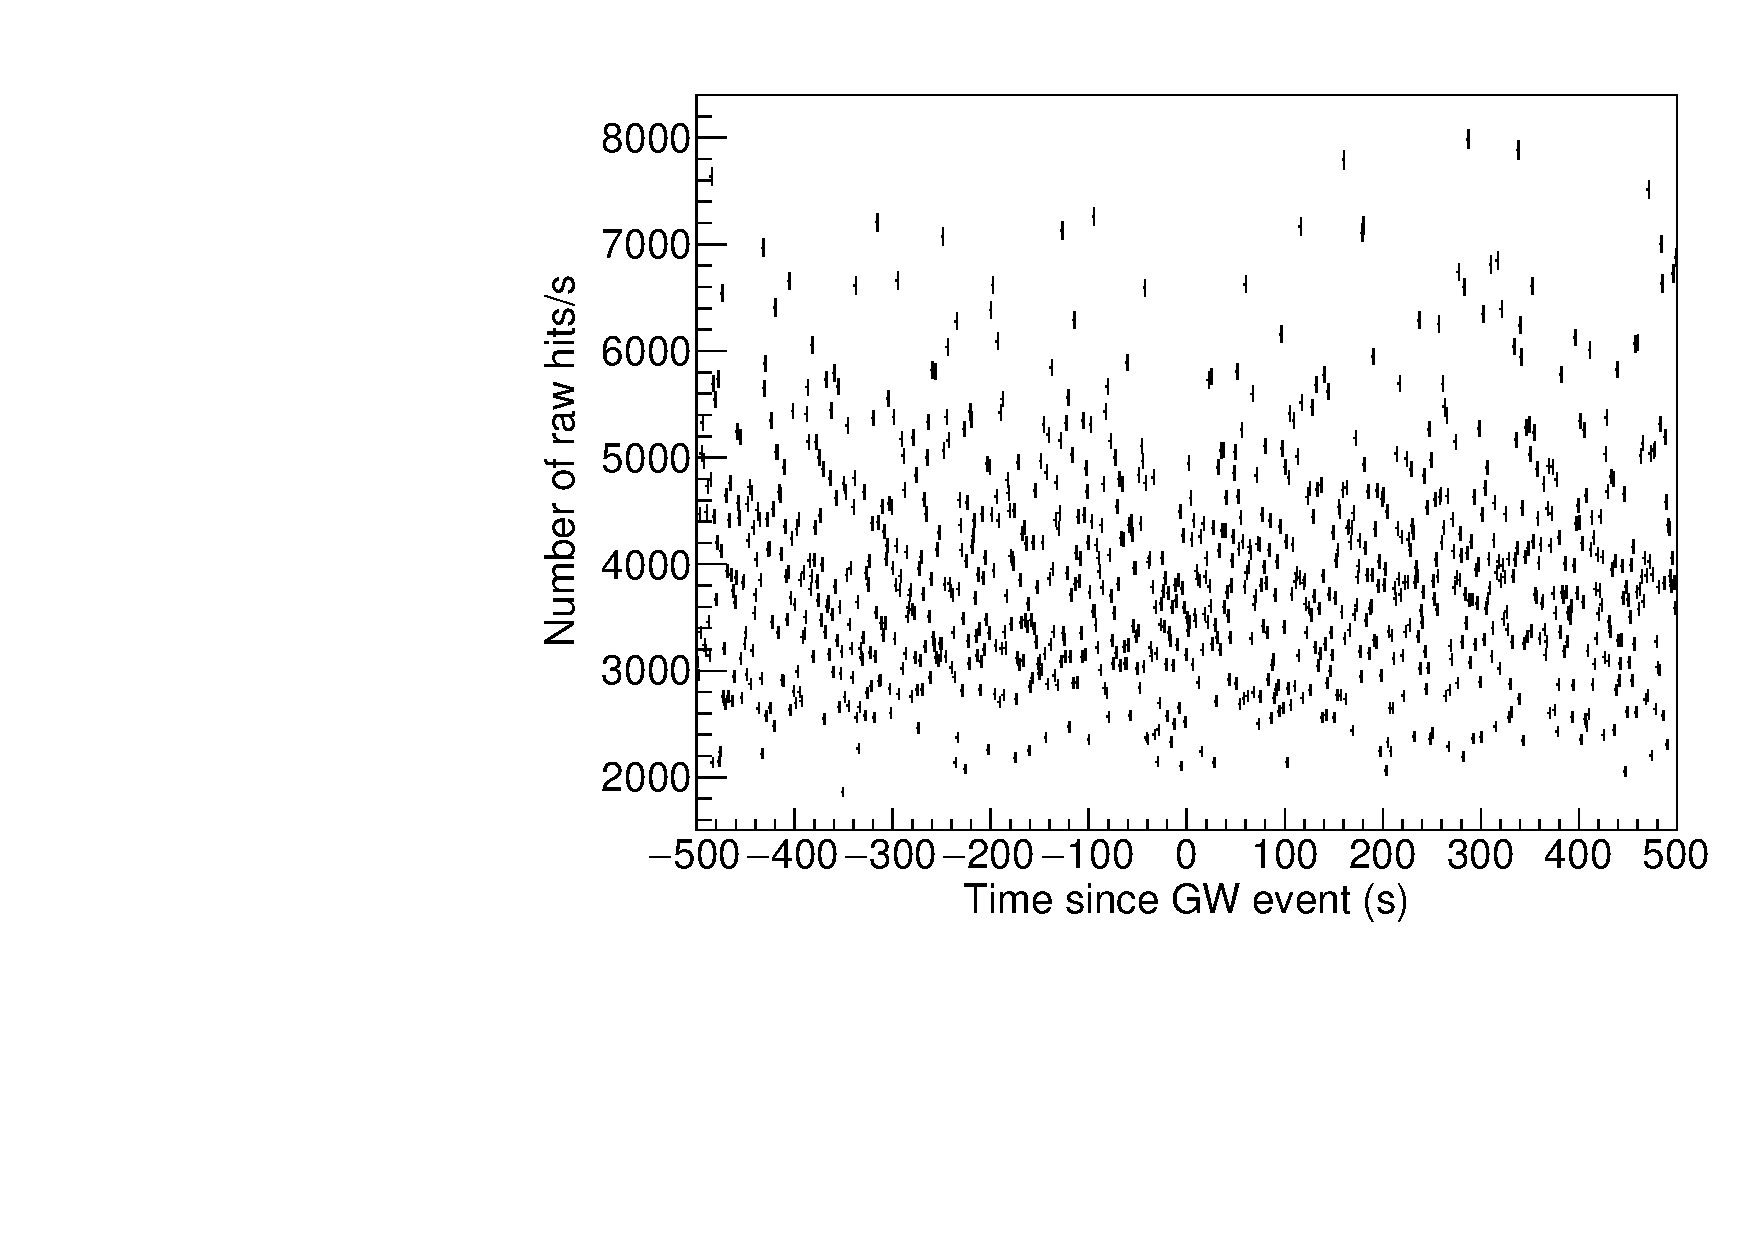
\includegraphics[width=0.333\columnwidth]{ligopass2-neardet-ddactivity1-rawhits.pdf}%
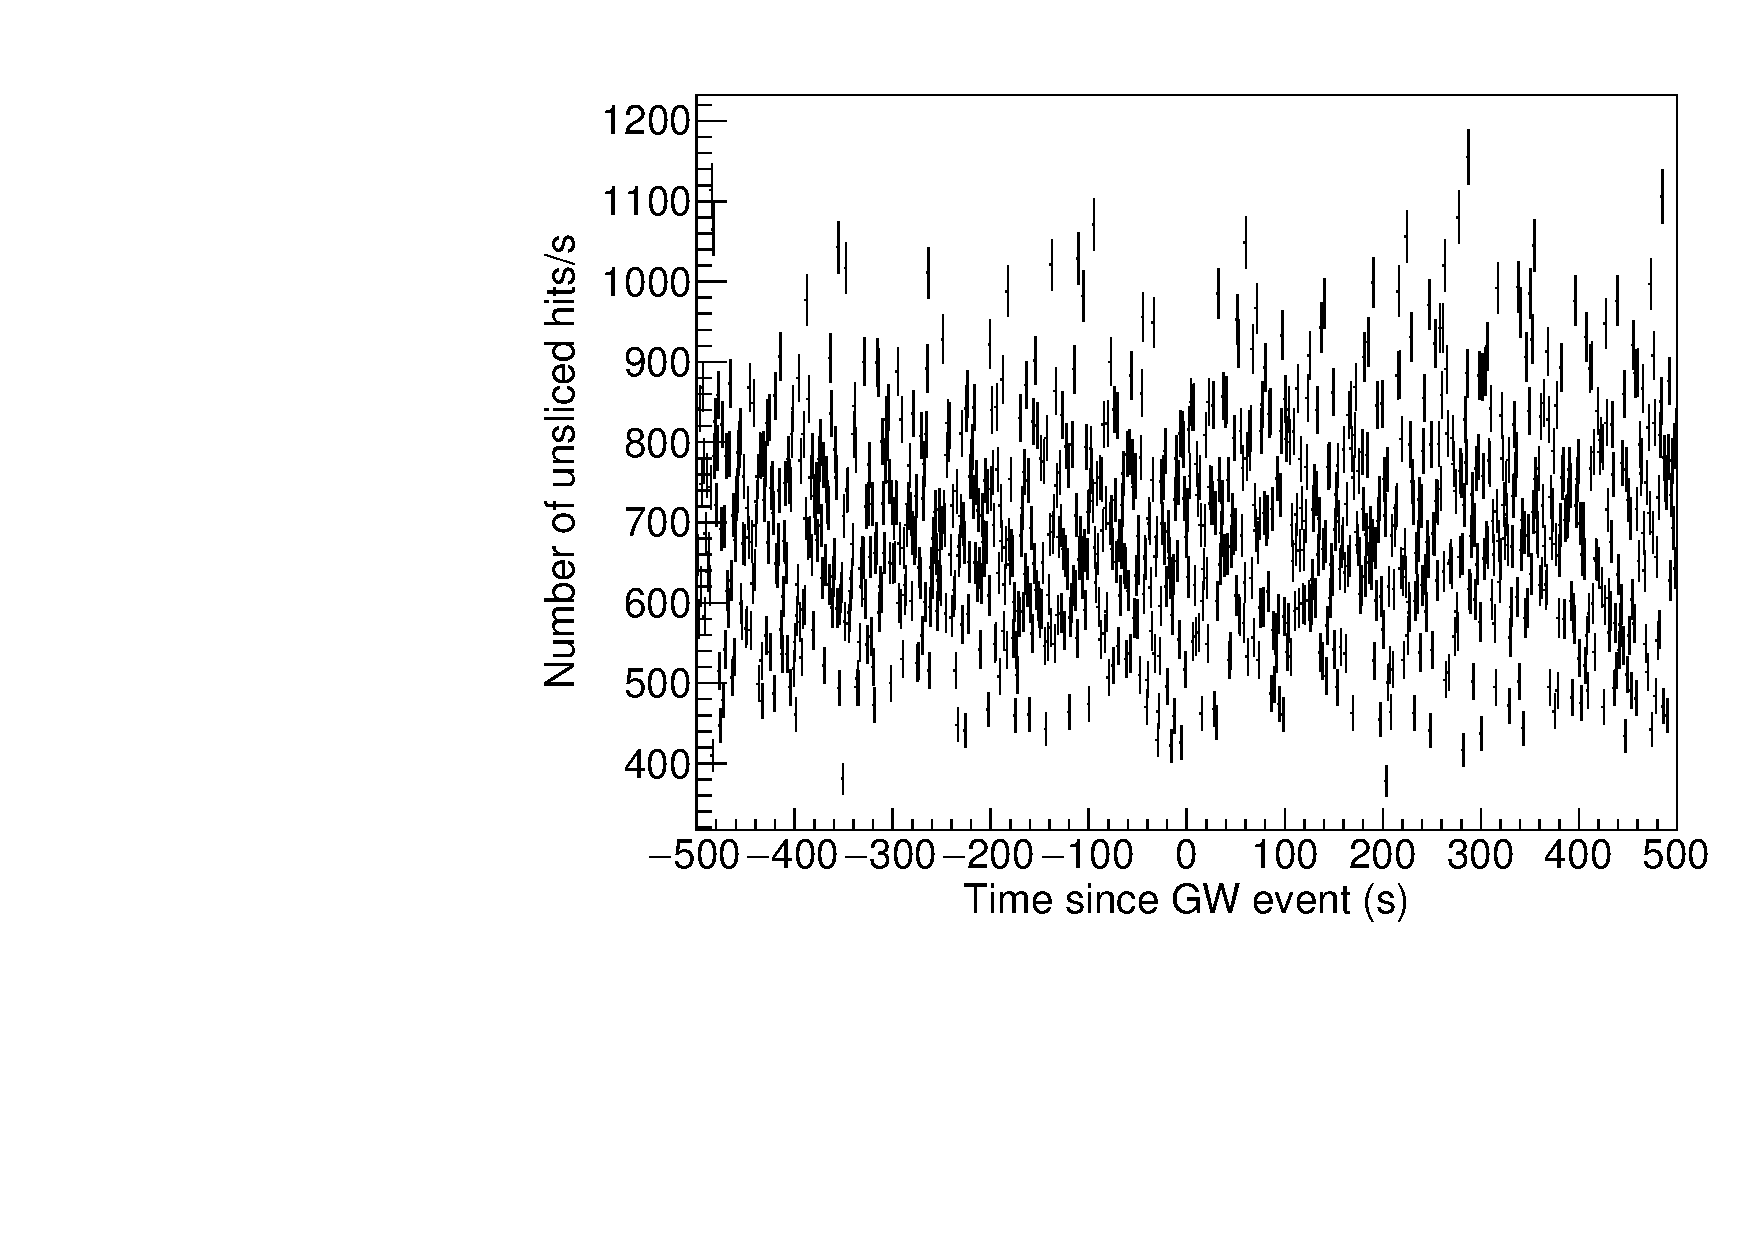
\includegraphics[width=0.333\columnwidth]{ligopass2-neardet-ddactivity1-unslicedhits.pdf}

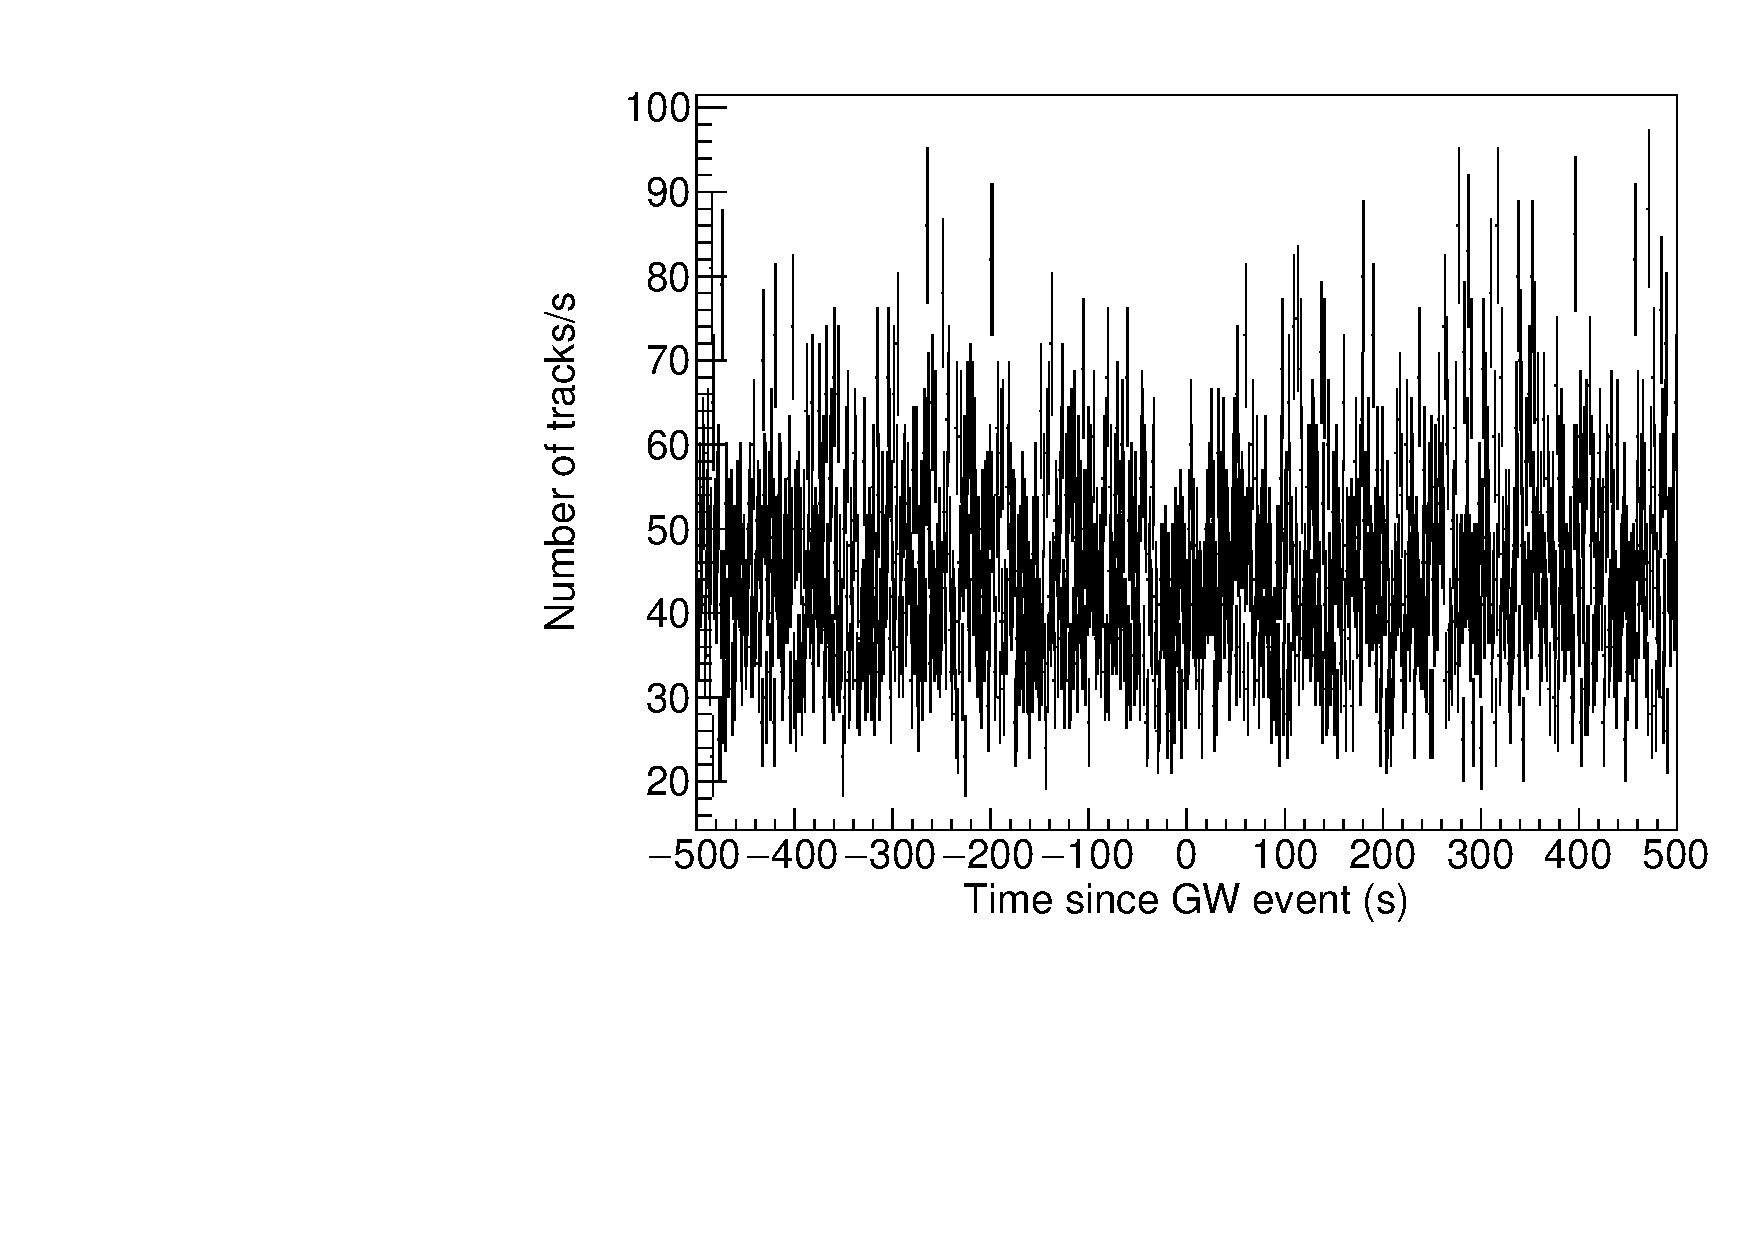
\includegraphics[width=0.333\columnwidth]{ligopass2-neardet-ddactivity1-tracks.pdf}%
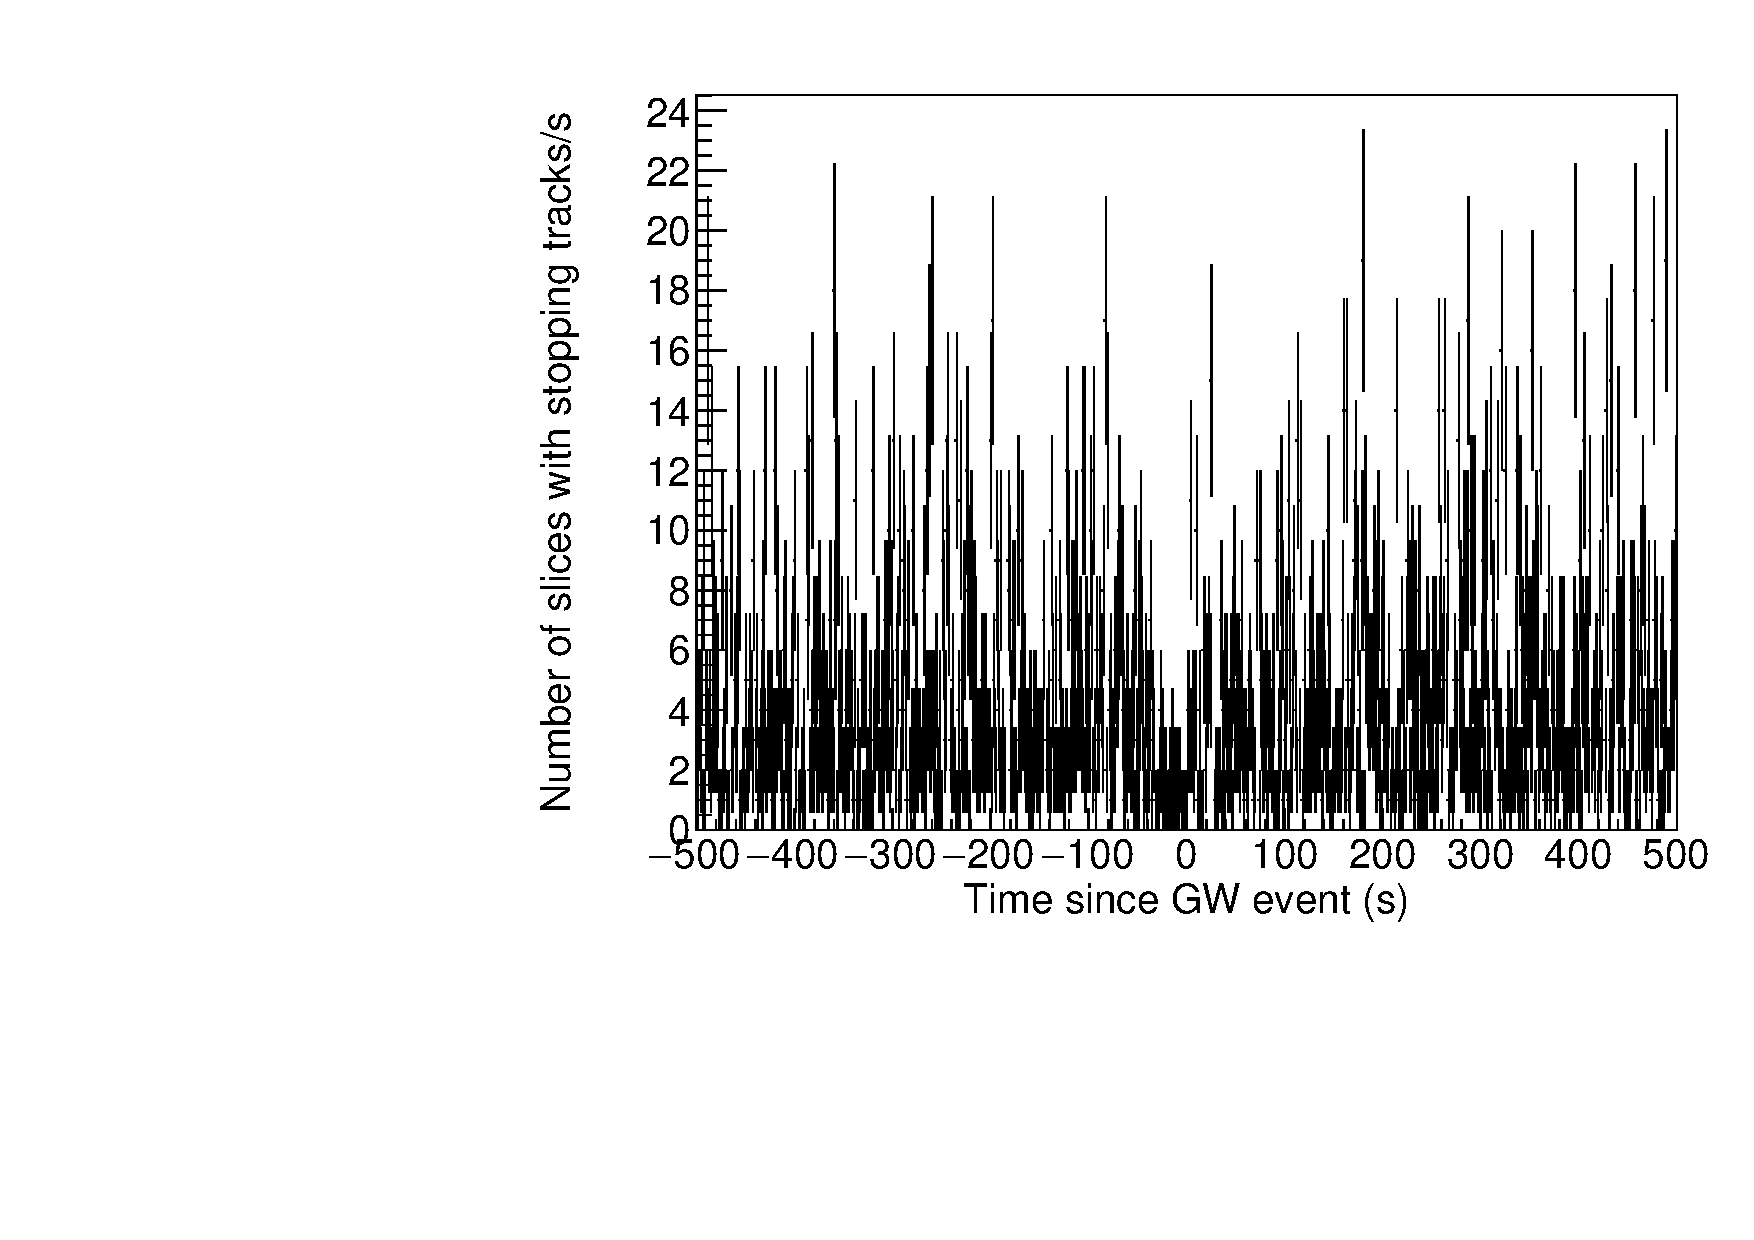
\includegraphics[width=0.333\columnwidth]{ligopass2-neardet-ddactivity1-stoppingtracks.pdf}%
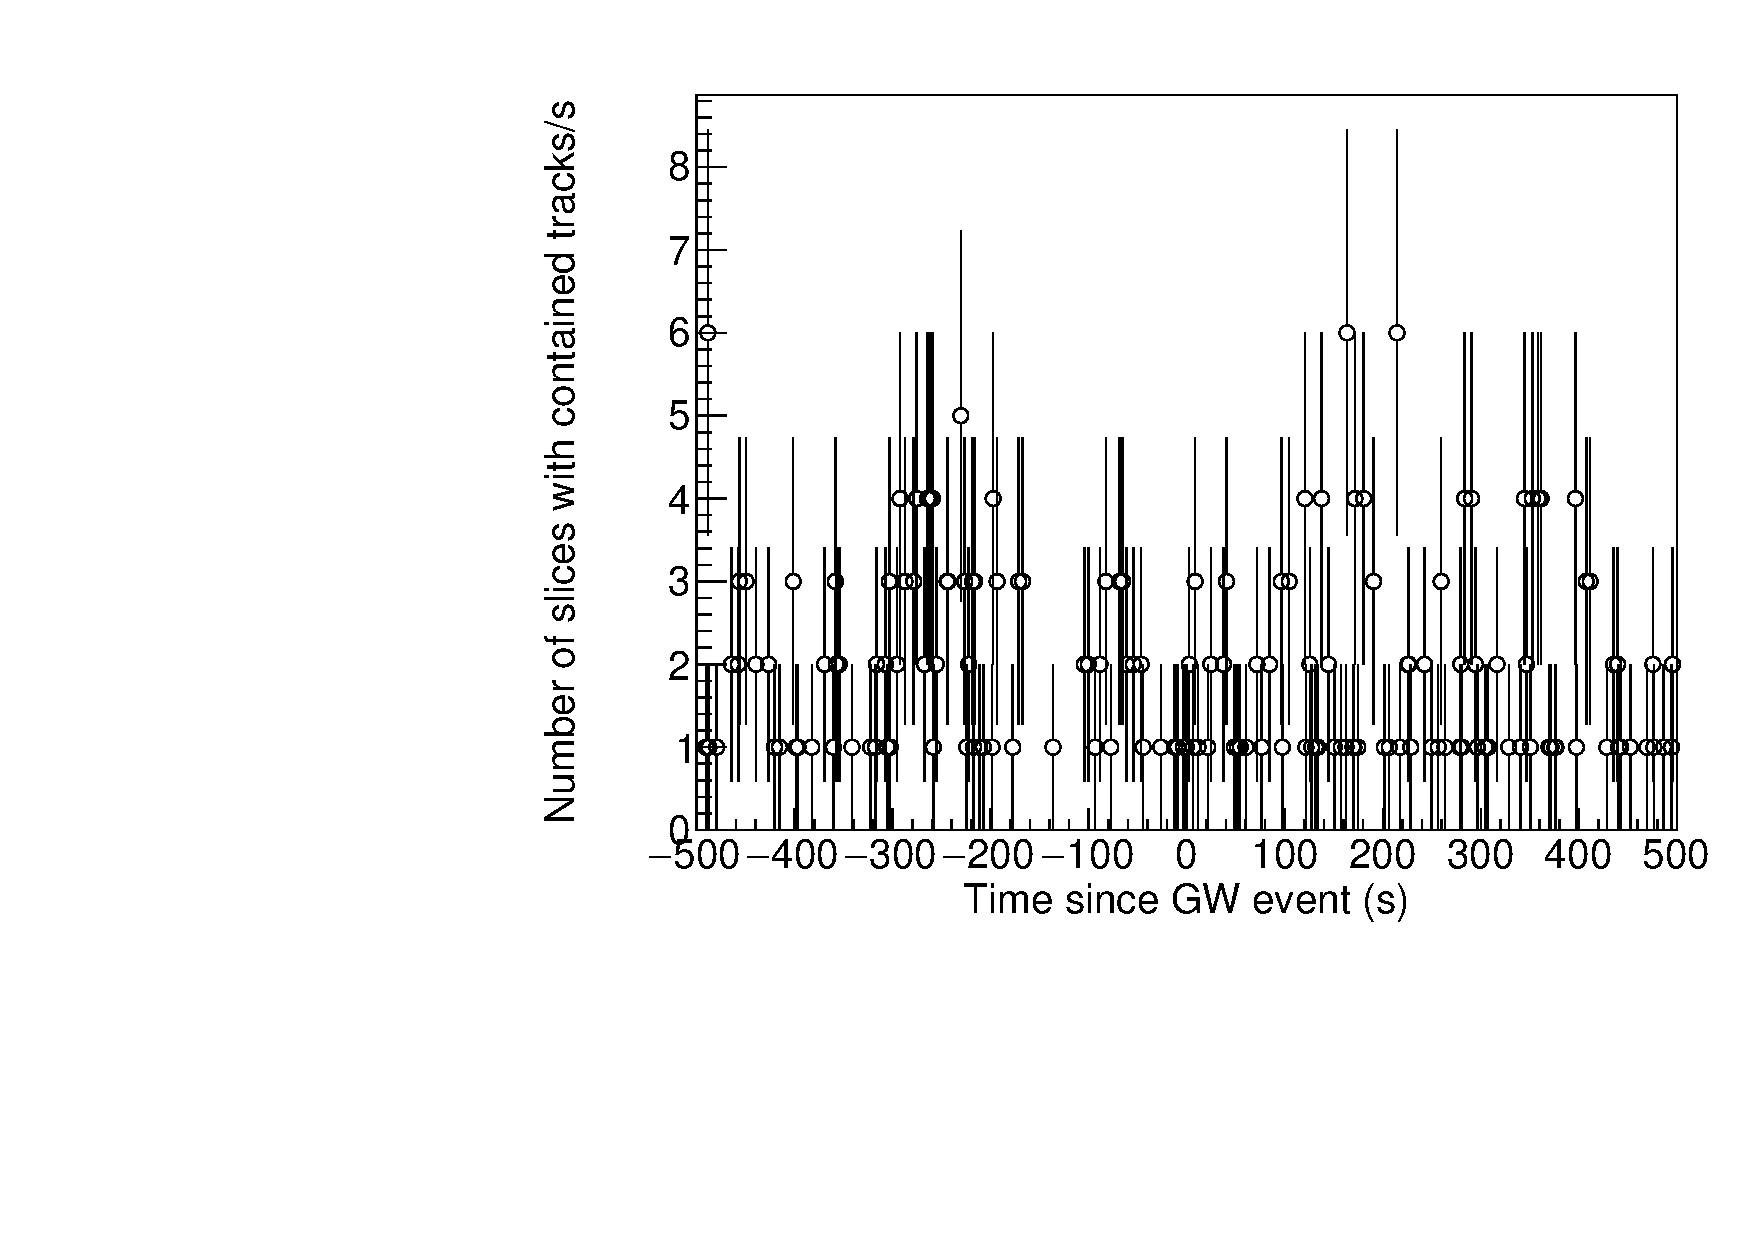
\includegraphics[width=0.333\columnwidth]{ligopass2-neardet-ddactivity1-containedtracks.pdf}%

\end{center}

\ul

  \item \alert{Not} dividing by livetime for this trigger

\lu

}


\section{To do}

\frame{\frametitle{To do}

\ul

\item Flesh out/refine the set of cuts and histograms for each trigger

\ul

  \item Plenty missing currently, e.g. nothing selects contained showers

  \item Want a much better analysis of MeV-scale events.  Will try DDsupernova's 
        slicer

\lu

\item Fit histograms to extract limits

\ul
\item Understand what the acceptance of each trigger is $\Rightarrow$ translate
 raw event count limits to something physical
\lu

\item Repeat test on O(50) randomly chosen times

\item Request box opening

\item Write paper

\lu

}

\beginbackup

\section{Backup}

\frame{\frametitle{Backups}}

\frame{\frametitle{So far}

\begin{center}
\begin{tabular}{c c c c c c}
\hline
\hline
Name & Time & ND & FD & Type & Pointing \\
\hline

 GW150914 & \phantom{0}9:50:45.4\phantom{00} & Good & {\color{orange}Ratty} & BH+BH & Rough \\
LVT151012 & \phantom{0}9:54:43\phantom{.000} & Good & {\color{red}Down}  & BH+BH & Rough \\
 GW151226 & \phantom{0}3:38:53.648           & Good & Good  & BH+BH & Rough \\
 GW170104 & 10:11:58.6\phantom{00}           & Good & Good  & BH+BH & Rough \\
 GW170608 & \phantom{0}2:01:16.49\phantom{0} & Good & Good  & BH+BH & Rough \\
 GW170814 & 10:30:43.53\phantom{0}           & Good & Good  & BH+BH & Good  \\
 GW170817 & 12:41:04.4\phantom{00}           & Good & Good  & NS+NS & Good  \\
\hline
\hline
\end{tabular}
\end{center}

}
\backupend
%%%%%%%%%%%%%%%%%%%%%%%%%%%%%%%%%%%%%%%%%%%%%%%%%%%%%%%%%%%%%%%%%%%%%%%%
\end{document}
